\documentclass{article}

\usepackage{arxiv}

\usepackage[utf8]{inputenc} % allow utf-8 input
\usepackage[T1]{fontenc}    % use 8-bit T1 fonts
\usepackage[hidelinks]{hyperref}       % hyperlinks
\usepackage{url}            % simple URL typesetting
\usepackage{booktabs}       % professional-quality tables
\usepackage{amsmath,amssymb,amsthm}
\usepackage{amsfonts}       % blackboard math symbols
\usepackage{float}
\usepackage{nicefrac}       % compact symbols for 1/2, etc.
\usepackage{microtype}      % microtypography
\usepackage{mathrsfs}
\usepackage{onimage}
\usepackage{graphicx}
\usepackage{doi}
\usepackage{acronym}
\usepackage{listings}
\usepackage[mode=buildnew]{standalone}
\usepackage{tikz}
\usepackage{tabularx}
\usepackage{siunitx}
\usepackage{cite}
\usepackage{acronym}
\usepackage{xcolor}

\usetikzlibrary{calc}
\usetikzlibrary{shapes.geometric, arrows}

\tikzstyle{rect} = [
    rectangle,
    align=center,
    minimum width=3.1cm,
    minimum height=1cm,
    text centered,
    fill=color4!40,
    draw=color4dark,
    line width=1pt,
]
\tikzstyle{frect} = [rect, fill=color5!40, draw=color5dark]
\tikzstyle{brect} = [rect, fill=color1!40, draw=color1dark]
\tikzstyle{arrow} = [line width=1.2pt,->,>=stealth]
\tikzstyle{darrow} = [arrow, dashed]

\definecolor{color1}{HTML}{6bd2db}
\definecolor{color1dark}{HTML}{56a9b0}
\definecolor{color2}{HTML}{0ea7b5}
\definecolor{color3}{HTML}{0c457d}
\definecolor{color3dark}{HTML}{09325c}
\definecolor{color4}{HTML}{ffbe4f}
\definecolor{color4dark}{HTML}{cc993f}
\definecolor{color5}{HTML}{e8702a}
\definecolor{color5dark}{HTML}{ba5922}


\title{Methods for Analyzing Models of\\ Rod-Shaped Bacteria}

%\date{September 9, 1985}	% Here you can change the date presented in the paper title
%\date{} 					% Or removing it

\author{
    \href{https://orcid.org/0009-0001-0613-7978}{
        
\includegraphics[scale=0.06]{figures/orcid.pdf}
        \hspace{1mm}Jonas Pleyer
    }
    \thanks{
        \href{https://jonas.pleyer.org}{jonas.pleyer.org},
        \href{https://cellular-raza.com}{cellular-raza.com}
    }\\
	Freiburg Center for Data-Analysis and Modeling\\
	University of Freiburg\\
	\texttt{jonas.pleyer@fdm.uni-freiburg.de} \\
	%% examples of more authors
	\And
	\href{https://orcid.org/0000-0002-6371-4495}{
        
\includegraphics[scale=0.06]{figures/orcid.pdf}
        \hspace{1mm}Christian Fleck
    }\\
	Freiburg Center for Data-Analysis and Modeling\\
	University of Freiburg
}

\newacro{abm}[ABM]{Agent-Based Model}
\newacro{ode}[ODE]{Ordinary Differential Equation}
\newacro{pbr}[PBR]{Physically-Based Rendering}

% Uncomment to remove the date
%\date{}

% Uncomment to override  the `A preprint' in the header
\renewcommand{\headeright}{Preprint}
%\renewcommand{\undertitle}{Technical Report}
\renewcommand{\shorttitle}{Methods for Analyzing Models of Rod-Shaped Bacteria}

\usepackage{enumitem}
\setlist{nolistsep}

%%% Add PDF metadata to help others organize their library
%%% Once the PDF is generated, you can check the metadata with
%%% $ pdfinfo template.pdf
\hypersetup{
pdftitle={% TODO
},
pdfsubject={q-bio.NC, q-bio.QM},
pdfauthor={Jonas Pleyer, Christian Fleck},
pdfkeywords={},
}

% Change numbering of equations
% \numberwithin{equation}{section}

% MAKE TITLES IN THEOREMS BOLD
\makeatletter
\def\th@plain{%
  \thm@notefont{}% same as heading font
  \itshape % body font
}
\def\th@definition{%
  \thm@notefont{}% same as heading font
  \normalfont % body font
}
\makeatother

\begin{document}
\maketitle


%###################################################################################################
\begin{abstract}
    \aclp{abm} have become popular tools in the study of complex cellular systems.
    However, despite their popularity, it is often difficult to systematically estimate their
    parameters and perform advanced analyses e.g. using the profile-likelihood.
    In this work, we study the mechanical properties of rod-shaped bacteria and provide techniques
    for estimating their parameters and performing identifiability analysis on them.
    Our approach follows a blueprint of a modular framework which can be adapted to other research
    questions.
    We use time series of microscopic images as input data and incorporate advanced effects as the
    elasticity of the rod.
    The developed model serves as a generalized foundation to describe multiple species of
    rod-shaped bacteria such as \textit{E.Coli} or \textit{B.Subtilis}.
\end{abstract}

% keywords can be removed
% \keywords{}

\pagebreak
\renewcommand{\contentsname}{Table of Contents (remove before submission)}
\tableofcontents
\pagebreak

%###################################################################################################
\section{Introduction}

\acp{abm} have proven to be powerfull tools in the study of complex cellular systems.
They have been applied in various scenarios, such as cancer
research~\cite{Ghaffarizadeh2018,Cooper2020}, Immuno-Oncology~\cite{Karolak2021} or the modeling
of mechanical intercellular connections in plant cells.
By treating cells as individual entities, these tools allow researchers to think in terms of
cellular properties and processes thus allowing for a better understanding of the biological
reality.

Despite their popularity, \acp{abm} face multiple challenges in practise.
Constructing a fully working \ac{abm} simulation from scratch is an intricate process that requires
a large set of skills and time.
It is therefore common practise to reuse existing simulation tools, which brings along a number of
other problems.
Even if the existing tool is designed to be generalizable, it often comes with a pre-defined set
of parameters that need to be specified.
Furthermore, as we have discussed in our previous work~\cite{Pleyer2023}, these tools were most
often not designed to be flexible but rather built for specific purposes thus limiting their
generalizability.
% TODO citations
Typically researchers aim to estimate every individual parameter of their model.
This is achieved using methods such as the profile-likelihood and model reduction techniques.
% TODO citaitons
When it comes to \acp{abm} however, it is often only shown that the results which have been
generated by an \ac{abm} lead to the desired phenomenon which aligns with the observed biological
reality thus omitting to actually estimate the necessary parameters directly.
% TODO citations
This reduces the confidence in the constructed models and raises concerns with respect to the
validity of the obtained results.

In this work, we address these challenges using a general-purpose mechanical model for rod-shaped
bacteria.
Our approach provides various methods which can be combined to systematically estimate the
parameters of our model.
We deliberately distinguish between conceptually separate components within this framework.
This modularity highlights a "blueprint" which can be adapted and applied to other \acp{abm}.

Mechanical properties of rod-shaped bacteria have been studied
extensively~\cite{Chatterjee1988,Takeuchi2005,IWAI2002}.
It was found that the MreB protein is the driving force in maintaining their distinct elongated
shape~\cite{Ursell2014}, which plays an important role in the dynamics of
growth~\cite{Billaudeau2017}, division~\cite{Harry2001} and their collective
behaviour~\cite{vanGestel2015}.
Furthermore, it has been discovered that the rod can be bent thus introducing temporary elastic or
permanent plastic deformations~\cite{Amir2014_2}.
They are an interesting target system since their physical form provides more surface information
compared to spherical cells.
In addition, parameters such as growth rates have been found to vary across multiple
cells~\cite{Koutsoumanis2013} which highlights the need to incorporate this heterogeneity on a
single-cell level.

Computational models for rod-shaped bacteria allow researchers to systematically analyze their
properties and infer emerging phenomena~\cite{Cho2007,Jnsson2005}.
Existing tools can describe growth, division and many effects such as colony formation and
expansion~\cite{Matyjaszkiewicz2017,Doumic2020} but they are limited in describing the
aforementioned plastic or elastic deformations of the rod.
Furthermore, the literature on how to estimate the parameters of such models is very sparse.

This work adresses some of these limitations.
We use microscopic image time series as inputs to obtain information about the spatial
configuration of the cells.
This information can be used as initial values for a numerical simulation.
By varying the parameters of the model and comparing the results to the microscopic data, we can
estimate and quantify the parameters of our model.
Our approach takes a general stance which incorporates effects that are observed within
\textit{B.Subtilis} and \textit{E.Coli}.

% General comments on \acp{abm} and their problems
\begin{itemize}
    \item \aclp{abm} are used for many purposes
    \item describe current way of estimating parameters; compare distributions to each other; no idea if
          individual parameters are correct
    \item challenge: estimate their parameters
    \item challenge: construct minimal models (requires flexibility)
\end{itemize}

General remarks about the steps in this work
\begin{itemize}
    \item Use rod-shaped bacteria as model system
    \item Clear separation between different components (link to overview)
    \item This separation allows us to generalize the type of approach and apply to other models
    \item think of as a "blueprint" for estimating parameters for \acp{abm}
\end{itemize}

Experimental observations: rod-shaped bacteria
\begin{itemize}
    \item growth + division "distinct mechanical properties", MreB
    \item bendiness (not much studied)
    \item individual parameters (i.e. growth rates)
    \item adhesion to each other
\end{itemize}

Computational studies of rod-shaped bacteria
\begin{itemize}
    \item not so many models for rod-shaped bacteria
    \item could include more effects such as bending
    \item almost no efforts to estimate parameters with individual-based models
    \item although many things known no "generalized mechanical model" constructed for rod-shaped bacteria
\end{itemize}

\section{Introduction (old)}

The last decades have fundamentally challenged and changed our understanding of how bacteria retain
their shape.
They exist in many physical forms such as spheroidal, rod-shaped or
spiral~\cite{Zapun2008,Young2006}.
Rod-shaped bacteria can grow by extending their cylindrical part, or by inserting new material at
the tip of the rod.
Species such as \textit{E.coli} and \textit{B.subtilis}~\cite{Errington2020} fall under the first
category while \textit{S.pombe} represents the latter.
New material is inserted in small bursts on the nanoscale in forms of patches, bands or
hoops~\cite{DePedro2003}.
Despite their differences such as wall-size or length \textit{B.subtilis} and \textit{E.coli} follow
growth rules which are comparable with respect to the extension of the rod~\cite{Chang2014}.

\paragraph{Experimental studies of mechanical properties}
It was long believed that bacteria lack cytoskeletal filaments but with the end of the last
century, it was discovered that the MreB protein fills this role since it "[..] forms an actin-like
cytoskeleton in bacteria [..]" \cite{Erickson2001}.
It can polymerize and form filaments which behave similar to actin microfilaments \cite{Dersch2020}.
Studies of its crystal structure further showed the similarity to actin \cite{vandenEnt2001} and the
MreB, MreC and MreD proteins were identified as homologues of actin \cite{Lowe2017_lj}.\
Jones et al. studied the species of different bacterial sub-kingdoms which have the MreB
gene~\cite{Jones2001}.
They concluded: "Many of the organisms are rod shaped, similar to \textit{B. subtilis} and
\textit{E. coli}.
Organisms with more complex shapes, including curved, filamentous, and helical bacteria, were all
abundantly represented." \cite{Jones2001}.
Furthermore, \cite{Wachi1987} found that mutants of \textit{E.Coli} which create defective MreB
proteins will be spherical instead of their natural rod-shaped form.

% \begin{itemize}
%     \item \cite{Robert2014} growth of individual rods, distribution of parameters
%     \item \cite{Koutsoumanis2013} inheritance of growth rates, growth parameter distributions
%     \item \cite{Ursell2014} MreB acts againts curvature during growth of cell
%     \item \cite{Takeuchi2005} cells in microchambers leads to plastic deformations
%     \item \cite{Amir2014} bending stiffness, plastic + elastic deformations
% \end{itemize}
Other experiments found that individual rods of \textit{E.Coli} grow exponentially until the
division event which is triggered by a size-sensing rather than a time-sensing
mechanism~\cite{Robert2014}.
These results also showed that the growth parameters were randomly distributed but did not quantify
said distribution.
Using $220$ \textit{Salmonella enterica}, Koutsoumanis et al. analysed the distribution of division
times and was able to quantify their distributions~\cite{Koutsoumanis2013}.
They found that while the initial division times were longer, there was no correlation between
division times of mother and daughter cells.
The first finding can be explained by the bacterias lag-phase~\cite{Bertrand2019} which is a
temporary period during which bacteria do not grow.
The second observation is an example of principle of thought which underlyies guides this work:
Cells are individual agents with individual parameters and thus individual behaviour and need to be
treated as such.
This is especially important if we want to determine parameters of our model for individual agents.

% \paragraph{Collective Effects \& Self-Organization}
% are emergent phenomena that result from the combined interactions of multiple cells.
% Although they do not allow us to fundamentally understand, the individual behaviour of cells
% directly, they can provide a way to falsify our results and thus further guide our modeling
% approach.
% \cite{Trejo2013} investigated the mechanical response of a tightly packed colony of \textit{Bacillus
% Subtilis}.
Trejo et al. studied the formation of macroscopic wrinkles when growing bacteria in a confined
space~\cite{Trejo2013}.
They were able to model the strain and stress of the collection of bacteria which requires that
cells are connected by a (to first order) spring-like force.
The developing wrinkles could then be described by a buckling instability.

Duvernoy et al. used laser techniques and force microscopy to investigate adhesion of individual
\textit{E.coli} and \textit{Pseudomonas aeruginosa} cells~\cite{Duvernoy2018}.
They found that the adhesion forces of the rods are polar, resulting in mechanical tension which in
turn determines daughter cell arrangement.
% They measured the size of the grown bacterial colonies, fitted ellipses to their shapes and found
% that adhesion and polar adhesion in particular resulted in a greater difference between the long and
% short axis of the fitted ellipse and thus a more oval shape rather than circular (WT).
By extending the work of \cite{Grant2014}, they further showed, that the critical value of
transitioning from a monolayer to multiple layers of bacteria, depends on the adhesive strength and
polarity of the interaction.
Grant et al. described the growing bacterial colony as a disc with radius $R$ which is pressed
into the agarose slab~\cite{Grant2014}.
The authors created a purposely-designed simulation in `C++` in order to model the effects of the
gel on the collection of bacteria.

Van Gestel et al. explored how \textit{B.subtilis} migrates over a surface by forming multicellular
structures~\cite{vanGestel2015}.
The cells organize themselves into "van Gogh bundles" of cells which are tightly aligned in chains
and form filamentous loops.
This phenomenon occurs at the border of the bacterial colony and the migration is driven by two
phenotypically different cell types~\cite{Lpez2010}.
% \begin{itemize}
%     \item \cite{Trejo2013} mechanical response of bacterial colony
%     \item \cite{Duvernoy2018} bacterial colonies form multilayers, interactions are polar
%     \item \cite{vanGestel2015} van Gogh bundles form from interplay of 2 cell-types
% \end{itemize}

\paragraph{Computational Modeling Frameworks which support Rod-Shaped Bacteria}
% \textbf{Requirements}
% \begin{itemize}
%     \item capture bendiness; do not assume rigid bodies
%     \item model in 2D and 3D possible
%     \item individual-based model; model single cells
%     \item collective phenomena; describe many interacting cells, not just a single one
% \end{itemize}
There have been many variations in modeling rod-shaped bacteria.
In order to provide enough flexibility and generality, we are in particular interested in models
that can capture non-rigid rods and work both in 2D and 3D scenarios.
Furthermore, we require that our model can describe bacteria individually and that a collective
model is simply the propduct of multiple individual agents interacting with each other.
In order to be able to investigate more specialized models, we need to be able to adjust and modify
any existing model.

In general, there are two classes of existing models which could be considered to fit these
criteria: purpose-built (onf-off) solutions and computational modeling frameworks which have been
designed to provide predefined cellular representations for various use-cases~\cite{Pleyer2023}.
However, explicit support for rod-shaped bacteria is rather sparse.
Biocellion has support for cylindrically-shaped agents but does not provide any mechanisms of how to
model bendiness or flexibility of the rod~\cite{Kang2014}.
BSim2.0 represents cells as rigid capsular cells made from a cylindrical center part and two
half-spheres, which are placed at the ends of the cylinder to round out the
shape~\cite{Matyjaszkiewicz2017}.
In order to calculate interactions between cells, possible overlaps are determined and minimized,
thus determining the position values of the next iteration step.
However BSim does not consider bending of the rods.
The \texttt{gro} programming language was designed to simulate the growth of colonies and cell-cell
communication~\cite{Gutirrez2017}.
Its “physics computation has been optimized for rigid rod-shaped bodies, like E. coli
bacteria”~\cite{Gutirrez2017}.
They recognize two types of forces which are acting on the cellular agents:
Local forces which are calculated between adjacent bacteria and a global force which pushes bacteria
outwards of the colony.
The latter of these is a phenomenological implementation of the observed colony expansion and the
associated central pressure with it.
This assumption may yield incorrect results for sparsely populated cases.
The engine is limited to 2D and does not consider polar interactions or bending of the rods.

% \textbf{Computational Modeling Frameworks}
% What has been done so far?
% \begin{itemize}
%     \item In general: not many frameworks which support some form of rod-shaped bacteria
%     \item \cite{Kang2014} Biocellion has support for cylindrically-shaped agents; no
%         bendiness/rigidity or polar interactions
%     \item \cite{Matyjaszkiewicz2017} BSim2.0 represents cells as rigid capsular cells made from a
%         cylindrical center part and two half-spheres, which are placed at the ends of the cylinder
%         to round out the shape. In order to calculate interactions between cells, possible overlaps
%         are determined and minimized, thus determining the position values of the next iteration
%         step.
%         BSim does not consider bending forces for individual cells or polar interactions.
%     \item \cite{Gutirrez2017} The gro programming language was designed to simulate the growth of
%         colonies and cell-cell communication. Its “physics computation has been optimized for rigid
%         rod-shaped bodies, like E. coli bacteria” (Gutiérrez et al. 2017). They recognize two types
%         of forces which are acting on the cellular agents: Local forces which are calculated between
%         adjacent bacteria and a global force which pushes bacteria outwards of the colony. The
%         latter of these is a phenomenological implementation of the observed colony expansion and
%         the associated central pressure with it. This assumption may yield incorrect results for
%         sparsely populated cases.
%         The engine is limited to 2D and does not consider polar interactions or bending of the rods.
% \end{itemize}

\paragraph{Applications \& Parameter Estimation}
% \begin{itemize}
%     \item \cite{Winkle2017} Modeling mechanical interations in growing populations of rod-shaped
%         bacteria
%     \item \cite{Doumic2020} "A purely mechanical model with asymmetric features for early
%         morphogenesis of rod-shaped bacteria micro-colony"
%     \begin{itemize}
%         \item Really good paper for referencing
%         \item comparison of distributions; not individual agents
%         \item no bending in model
%         \item uses steric force (see also \cite{Trejo2013})
%     \end{itemize}
%     \item \cite{Grant2014} purposely-built model written in C++
%     \begin{itemize}
%         \item describes bacteria as collection of overlapping spheres
%         \item spheres are coupled by non-linear springs (Euler-Bernoulli dynamic beam theory). This
%             assumption is werid but does not alter their results
%         \item Only model repulsive forces; no attraction, adhesion
%     \end{itemize}
%     \item \cite{Cho2007} only 2D model; no param estimation; based on work done in \cite{Jnsson2005}
%     \item \cite{Storck2014} no bending; 41 parameters for various cases; only 8 parameters taken
%         from literature values or quantified; generate growth rate from normal distribution at each
%         integration step; stochastically equivalient for collection of bacteria but unfounded for
%         individual bactera
%     \item \cite{You2018}
% \end{itemize}

Cho et al.~\cite{Cho2007} extended the work done by~\cite{Jnsson2005} and construct a 2D model to
study self-organization of colonies within restricted geometries of microfluidic devices.
They do not provide any estimates of the parameters that were used.

You et al. assumed a hard-rod model to study the emergence of order within microdomains  of
rod-shaped bacteria~\cite{You2018}.
They were able to show that the hydrodynamic equations of active nematic liquid crystals can serve
as a continuum limit of their model.

Winkle et al. represented cells with "[..] two acially independent cell halves that attach through a
compressible, stiff spring [..]"~\cite{Winkle2017} and leveraged parts of the \texttt{gro}
infrastructure.
However, they only discuss results qualitatively without quantifying any of the used parameters.

Doumic et al. constructed a model which takes into account asymmetries of the individual bacteria
such as length, weight and friction~\cite{Doumic2020}.
They were able to estimate some of the used parameters by comparing distributions of simulated data
to distributions of experimental data.
However, in doing so, no optimization optimization methods were used, but parameters were picked by
hand in an attempt to best fit the observed results.
Furthermore, their model is not able to describe any deformations such as bending of the rods.

Grant et al. designed a custom \texttt{C++} program to simulate individual
bacteria~\cite{Grant2014} which are represented as elastic rods of overlapping spheres.
Their model does not include any attractive forces between agents but is able to describe bending of
the rods in 2D and 3D.
When it comes to the task of estimating parameters of the model, values are picked by hand in order
to mimick the observed experimental results.

Storck et al. constructed a flexible model which is based on particles and springs and thus able to
describe a variety of cells~\cite{Storck2014}.
Since this model incorporates many effects, it consists of $41$ parameters of which only $8$ have
values that are taken from litearture or otherwise quantified.
Another choice of their modeling approach was to stochastically assign growth bursts at each
integration step of the numerical solving process.
When generating from a normal distribution and observing on a collective level, this is
stochastically equivalent to picking and fixing growth rates for each cell from the same
distribution but is not identical when observing individual agents.

\paragraph{The missing Link}
It is clear that researchers are interested in studying mechanical properties of rod-like bacteria
in order to better understand phenomena such as biofilm formation.
The major downside of existing computational models is that there are almost no methods to properly
quantify their parameters which diminishes their explanatory power.
By leveraging a simple assumption about the cellular representation, this work aims to solve this
particular problem.



%###################################################################################################
\section{Overview}
This work consists of many subcomponents which can be combined in order to achieve various tasks.
Figure~\ref{fig:flowchart-project-structure} shows a high-level overview of all components.
We assume that bacterial rods can be represented by a colleciton of vertices $\vec{x}_i$.
This assumption alone is enough to enable a cascade of other components.
Using the spatial representation, we provide visualization methods that create 3D models from the
given vertices which can then either be rendered or projected to a 2D plane.
The data extraction component determines the vertices $\vec{x}_i$ from given cell masks which
correspond to microscopic images.
This allows us in particular to turn any sequence of images (movie) into a sequence of bacterial
positions.
The dynamics of the vertices $\vec{x}_i$ are determined by a computational model which is specific
to the respective use-case and should be defined by the researcher.
It merely needs to utilize the aforementioned spatial representation of bacterial rods as a
collection of vertices $\vec{x}_i$.
This work will provide one example of how such a model can be defined.
Notably, the visualization and data extraction components do not require any knowledge about the
computational model, thus allowing us to reuse their functionality across multiple models.

Constructing a computational model requires knowledge about the target system and thus allows us to
interpret the results gathered by the provided data extraction methods.
These results can then further be used to restrict or determine the parameters of our model.
For example, by extracing the positions of bacteria across a time-series of microscopic images, we
can also calculate their lengths at these time-points and thus determine their rate of growth and
type of growth (see section~\ref{subsec:parameter-estimation-individual-treatment}), thus
effectively guiding our modeling steps.

Visualization methods are an integral part of any modeling endevaour.
They allow researchers to obtain feedback quickly and improve iteration times when constructing new
models.
Furthermore, we utilize them in our more advanced parameter estimation methods (see
section~\ref{section:parameter-estimation}) where they enable us to effectively compare
two bacterial configurations across division events.
In the future, we are planning to build on the current state and generate realistic microscopic
images and time-series.
Together with the parameter estimation methods, they can then be used to provide large amounts of
mechanistic data for the training cell-segmentation and cell-tracking machine-learning algorithms.

% \begin{itemize}
%     \item This publication contains 5 things:
%     \begin{enumerate}
%         \item Methods of how to obtain data from microscopic images and perform parameter
%             estimations; $\rightarrow$ also possibly across multiple generations
%         \item Showcase the usefulness of the methods and the model by applying it to parameter
%             estimation via microscopic images and multilayer formation
%         \item Initial (incomplete) model of rod-shaped bacteria
%         \item Generate 3D Images (masks)
%         \item A python package which can do all of that and can be reused and extended
%     \end{enumerate}
%     \item Overall structure
%     \begin{enumerate}
%         \item users bring model + data
%         \item this paper provides methods to do the parameter estimation + visualization
%     \end{enumerate}
%     \item For complete model, more work has to be done
%     \begin{itemize}
%         \item More aspects (see Review; put in discussion)
%         \item Note that we only care about \textit{E.Coli} and \textit{B.Subtilits}! This is
%             important.
%     \end{itemize}
%     \begin{itemize}
%         \item State of the Art
%     \end{itemize}
% \end{itemize}

\begin{figure}
    \centering
    % \includegraphics[width=0.8\textwidth]{overview.pdf}
    \includestandalone[width=0.8\textwidth]{figures/concept/overview}
    \caption{
        The project can be divided into subcomponents (yellow, red) that interact with and depend on
        each other.
        Yellow blocks are provided by this work and red blocks require additional input such as
        modeling assumptions or data.
        Blue blocks indicate possible future extensions of this project.
        Every component implicitly builds on the spatial representation of rod-shaped bacteria as
        vertices $\vec{x}_i$.
    }
    \label{fig:flowchart-project-structure}
\end{figure}

%###################################################################################################
\section{Methodology}
% --------------------------------------------------------------------------------------------------
\subsection{Spatial Representation of Rod-Shaped Bacteria}
\label{subsec:spatial-representation}
This work makes use of a few but powerfull assumptions concerning the mathematical representation of
the cells in question.
In order to describe the spatial dynamics of individual agents, we need to define their position,
shape and how they interact with each other.
In order to provide as much flexibility as possible when constructing new models, we restrict
ourselves to assumptions concerning the position such that researchers can freely experiment with
various shapes and interaction types.
Furthermore, it is very important to strike a good balance between the restrictiveness of our
assumptions and generality in order to provide meaningful results and still be able to apply our
approach to a broader class of models.
Taking into account the natural shape of rod-like bacteria, it is clear that they can not be
represented with a singular point $\vec{x}$ in space.
We could extend this positional definition with a vector $\vec{w}$, indicating the direction of
extension but this would restrict ourselves to fully straight rod-shaped bacteria.
However, multiple experiments have shown that MReB is responsible for the growth and maintenance of
the elongated shape of bacteria~\cite{Erickson2001}.
By means of this protein, rod-shaped bacteria can bend elastically on short time-scales and
deform plastically over longer periods of time.
Our goal is to provide a model which can encapsulate these effects.
Thus, we extend our model from a single point to multiple vertices which are part of a 1-dimensional
polygon with two endpoints $\vec{x}_i$.
In essence, we discretize the (possibly non-straight) rod of the agent.
Figure~\ref{fig:mechanics-bacterium} shows a visualization of this approach.
The angles $\alpha_i$ between vertices $\vec{x}_{i-1},\vec{x}_i$ can be used when modeling the
dynamics of these bacteria.

With these fundamental thoughts layed out, we retain the flexibility to represent many models such
as varying shapes since we do not have to make any assumptions on the type of interactions between
two bacteria.
Even concerning the shape of bacteria, this assumption still allows us to mdoel elliptical cells by
modifying the interaction type as well as other effects such as polarity of
interactions~\cite{Duvernoy2018}.
Furthermore, we also did not have to assume any particular mechanical dynamics of the agents, only
their spatial representation, thus leaving in particular room for plastical or elastic deformations
of the rod and other more intricate mechanisms.

% \begin{enumerate}
%     \item represent bacteria as polygon with vertices $\vec{x}_i$
%     \item Assumes that these vertices are not fundamental but rather a discretization of the actual
%         problem
% \end{enumerate}

\begin{figure}
    \centering
    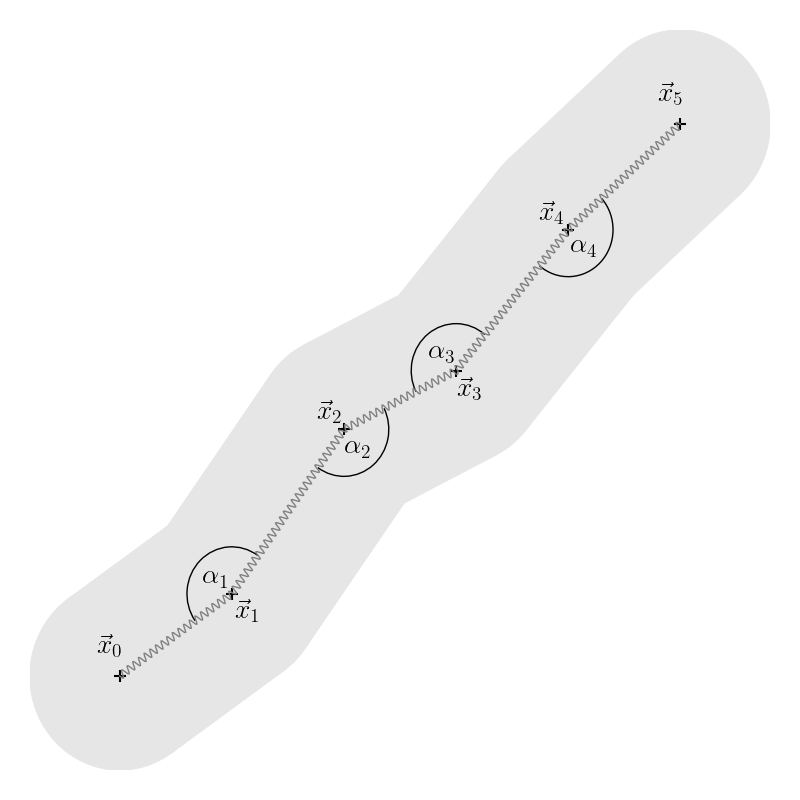
\includegraphics[width=0.5\textwidth]{docs/source/_static/mechanics.png}
    \caption{
        Example of an elonged bacterial rod represented by a collection of vertices which are
        connected by springs.
        The angles $\alpha_i$ have been exaggerated such that they can be identified more easily.
        A bacterial agent which is not interacting with any external objects will tend to the
        equilibrium state of a straight rod with $0$ curvature.
    }
    \label{fig:mechanics-bacterium}
\end{figure}

% --------------------------------------------------------------------------------------------------
\subsection{Visualization}
\label{subsection:visualization}

For visualization we use pyvista, which provides high-level wrappers around the popular VTK
library~\cite{vtkBook,Sullivan2019}.
The first stage of our visualization is to generate 3D meshes for each bacterium, which we consider
an intermediate representation.
We insert spheres of a given radius $r$ at each vertex $\vec{x}_i$ and connect adjacent vertices
$\vec{x}_i,\vec{x}_{i+1}$ with a cylinder, also of radius $r$ which is positioned such that its core
is identical to the connecting line segment between the two vertices.
Finally, we combine the meshes of all of these objects to obtain a single mesh of one bacterium.
A render of this result can be seen in figure~\ref{fig:progression-image-generation}.
Since we use a 3D rendering engine as an intermediate representation, the resulting image can have
overlaps of bacteria which are placed at higher or lower values along the z-direction.

To generate masks, we assign unique colors to every mesh of the respective cellular agent.
This mapping is unique, ensuring no two agents will use identical colors.
We then use a parallel projection and remove any existing light sources in order to obtain a solid
color for every cell-agent.
The resulting image is shown in subfigure (B).
Subfigure (C) shows an example of a simplified way to generate microscopic images.
The properties of the meshes such as roughness and reflectivity have been adjusted and we use
physically-based rendering of VTK.
The result of this render is augmented by introducing white noise on the pixel values at each point.
This approach is very rudimentary and we hope to extend these methods in the future.
In order to properly generate data, we need to deal with microscopic imaging techniques and possible
defects that can occurr.
It is crucial to get this part of the image-generation process right in order to obtain
near-realistic images that can be further reused.

% \begin{itemize}
%     \item use pyvista (VTK) for Visualization
%     \item always do 3D render. This way, we can have overalp between agents and produce more
%         realistic masks.
%     \item Assign unique color values for idividual agents.
%         We have a 1:1 mapping between agent identifier and color! (for each simulation different
%         though)
%     \item use parallel projection; this should be most close to what microscopes measure due to the
%         relatively large distance between object and lens.
%     \item use some noise to smear out the rods; this is already similar to microscopic images; use
%         more like this and deal with real-world defects to make it more realistic (future, not now)
%     \item Figure~\ref{fig:progression-image-generation} shows steps in generating image.
%     \item Reflectivity, placement of light etc. can already introduce some heterogeneity in the
%         visual of the rod.
%     \item Plan to implement noise on the mesh itself; make it have rough surface (like real rods as
%         seen under electron microscopy)
% \end{itemize}
%
% \paragraph{Algorithm}
% \begin{enumerate}
%     \item Get position of cell
%     \item Insert spheres at each vertex
%     \item Insert cylinder along edges
%     \item Combine individual objects into one big mesh
%     \item Use \ac{pbr}
% \end{enumerate}

\begin{figure}
    \centering
    % \begin{tikzonimage}[width=0.9\textwidth]{visualization.pdf}
    %     \node at (0.025, 0.975)[anchor=north west, rectangle, draw, minimum width=15pt, minimum height=15pt]{\textbf{A}};
    % \end{tikzonimage}
    \begin{tikzonimage}[width=0.3\textwidth]
        {docs/source/_static/09395645494836445480/raw_pv/000000400.png}
        \node at (0.025, 0.975)[anchor=north west, rectangle, draw, white, minimum width=15pt, minimum height=15pt]{\textbf{A}};
    \end{tikzonimage}
    \begin{tikzonimage}[width=0.3\textwidth]
        {docs/source/_static/09395645494836445480/masks/000000400.png}
        \node at (0.025, 0.975)[anchor=north west, rectangle, draw, white, minimum width=15pt, minimum height=15pt]{\textbf{B}};
    \end{tikzonimage}
    \begin{tikzonimage}[width=0.3\textwidth]
        {docs/source/_static/09395645494836445480/images/000000400.png}
        \node at (0.025, 0.975)[anchor=north west, rectangle, draw, white, minimum width=15pt, minimum height=15pt]{\textbf{C}};
    \end{tikzonimage}
    \caption{
        (A) shows the result from combining sphere and cylinder meshes to obtain the shape of a
        bacterial rod.
        This render contains lighting coming from 2 light sources which thus produces a small glow
        on the upper part of the meshes.
        (B) Unique color values are assigned to each agent and light sources are removed.
        Afterwards, the image is rendered by projecting along the z-axis.
        (C) We use physically-based rendering and assign properties such as roughness and
        reflectivity to generate an initial render.
        Afterwards, we apply white noise to the pixel values of image.
        In the future, we hope to extend this approach in order to construct near-realistic
        microscopic images from synthetic data.
    }
    \label{fig:progression-image-generation}
\end{figure}

% --------------------------------------------------------------------------------------------------
\subsection{Data Extraction}
\label{section:data-extraction}

This section will explain how we can determine the collection of vertices $\vec{x}_i$ introduced in
subsection~\ref{subsection:mechanical-model-mechanics} from microscopic images
(Figure~\ref{fig:position-extraction-algorithm} (A)).
They will serve as initial, final and intermediate values with which we can compare our predictions.
The algorithms which we devised requires the input of cell-masks which assign a unique color for
every cell in the image.
Such masks can be generated by cell-segmentation tools or obtained by annottating microscopic images
by hand (Figure~\ref{fig:position-extraction-algorithm} (B)).
Afterwards, we proceed with the following 5 steps.
\begin{enumerate}
    \item Obtain submasks for each cell individually.
    \item Skeletonize submask with algorithm from Lee~\cite{Lee1994}
    \item Determine endpoints $\vec{q}_0,\vec{q}_1$.
        Assert that there are only 2 endpoints.
    \item Sort points such that they form a polygon.
    \item Interpolate vertices $\vec{x}_i$ from obtained polygon.
\end{enumerate}
In the first step, the image will be split into a collection of subimages that only contain
information for one single cell.
From there, we apply a skeletonization algorithm~\cite{Lee1994}
(Figure~\ref{fig:position-extraction-algorithm} (C)).
It has to be noted that there are multiple variants of skeletonization and in general, these classes
of algorithms can produce results which have intersection points and multiple endpoints.
This described behaviour is undesirable in our case.
We have found that for most practical examples, the algorithm devised by~\cite{Lee1994} has worked
well.\\
The skeletonization algorithm supplies us with a collection of unordered lattice points $\vec{p}_i$
(pixel coordinates) where the skeleton lives.
We identify the endpoints $\vec{q}_0,\vec{q}_1$ by counting the number of neighbors in the von
Neumann neighborhood for each lattice point.
Any point with exactly one neighboring point must be and endpoint.
If we encounter more or less than two points which fit this criterion, the routine can not commence
and is aborted.
Next, we start with one of the endpoints and determine the next neighbor which was not yet picked.
We list the points in this order, thus forming a sorted polygon of pixel coordinates.\\
In the last step, we take the sorted, extracted points $\vec{p}_i$ and interpolate $n$ values for
the desired number of vertices $\vec{x}_i$.

\begin{figure}
    \centering
    \begin{tikzonimage}[width=0.36\textwidth]
        {docs/source/_static/fitting-methods/algorithm/image001042.png}
        \node at (0.025, 0.975)[anchor=north west, rectangle, draw, white, minimum width=15pt, minimum height=15pt]{\textbf{A}};
    \end{tikzonimage}
    \begin{tikzonimage}[width=0.36\textwidth]
        {docs/source/_static/fitting-methods/algorithm/mask-zoom.png}
        \node at (0.025, 0.975)[anchor=north west, rectangle, draw, white, minimum width=15pt, minimum height=15pt]{\textbf{B}};
    \end{tikzonimage}
    \begin{tikzonimage}[width=0.255\textwidth]
        {docs/source/_static/fitting-methods/algorithm/interpolate-positions.png}
        \node at (0.025, 0.975)[anchor=north west, rectangle, draw, white, minimum width=15pt, minimum height=15pt]{\textbf{C}};
    \end{tikzonimage}
    \caption{
        (A) Input image.
        (B) Result of the skeletonization algorithm for a single cell.
        (C) Vertices $\vec{x}_i$ which have been interpolated from the skeletonized cell.
        They represent the position of our cell-agents.
    }
    \label{fig:position-extraction-algorithm}
\end{figure}

% --------------------------------------------------------------------------------------------------
\paragraph{Benchmarking the Extraction Algorithm}
\label{paragraph-extraction-algorithm}

In order to determine if our extraction algorithm provides reliable results, we have to take
advantage of a functionality which will be introduced later in
section~\ref{subsection:visualization}.
Our methodology makes use of the fact that we have already set up our model and solving scheme and
are able to produce cell masks from these numerical results.
In doing so, we have exact knowledge about the position of our agents since we can simply obtain
this information from our model.
But on the other hand we can also try to extract this position from the generated cell-masks.
By comparing the differences between them, we get a good estimate of how well our extraction
algorithm can determine the true position of the bacteria.

In figure~\ref{fig:benchmarking-extraction-algorithm} (A-C) we see snapshots of a time series of
masks.
This particular simulation includes division events between images (B) and (C).
For all images (A-C), we have drawn the exact position of the agents with white lines and indicated
the extracted positions with crosses.
They align very well visually.
It may be hard to spot with the bare eye, but the agreement between extracted and exact positions is
visually worse at the endpoints of the rods.
To quantify this disparity, we calculate the distance between these individual vertices.
Figure~\ref{fig:benchmarking-extraction-algorithm} (D) shows the estimated length of the rods from
the extracted and exact vertices which is surrounded by the average vertex distance.
Division events lead to steps in our rod-length function since the bacterial length is halved.
We can clearly see that the agreement is very good in the beginning but right after every division
event, the uncertainty becomes large.
To illustrate this, we can see that in figure~\ref{fig:benchmarking-extraction-algorithm} (C) some
of the rods are partially overlapping which hides parts of the individual cell-masks and thus
changes the extraction result.
We also plotted the distribution of individual vertex distances in
figure~\ref{fig:benchmarking-extraction-algorithm} (E).
Darker areas in the plot correspond to distances at time-points earlier in the simulatin time.
We can see that brighter areas tend to shift towards the right, thus increasing the uncertainty of
the extraction.
However, the overall distribution shows small values of distances for a large number of vertices and
is not dominated by outliers.

\begin{figure}
    \centering
    \begin{tikzonimage}[width=0.32\textwidth]
        {docs/source/_static/fitting-methods/extract_positions-004000.png}
        \node at (0.025, 0.975)[anchor=north west, rectangle, draw, white, minimum width=15pt, minimum height=15pt]{\textbf{A}};
    \end{tikzonimage}
    \begin{tikzonimage}[width=0.32\textwidth]
        {docs/source/_static/fitting-methods/extract_positions-006000.png}
        \node at (0.025, 0.975)[anchor=north west, rectangle, draw, white, minimum width=15pt, minimum height=15pt]{\textbf{B}};
    \end{tikzonimage}
    \begin{tikzonimage}[width=0.32\textwidth]
        {docs/source/_static/fitting-methods/extract_positions-008000.png}
        \node at (0.025, 0.975)[anchor=north west, rectangle, draw, white, minimum width=15pt, minimum height=15pt]{\textbf{C}};
    \end{tikzonimage}
    \begin{tikzonimage}[width=0.5\textwidth]
        {docs/source/_static/fitting-methods/displacement-calculations.png}%
        \node at (0.03, 0.99)[anchor=north west, rectangle, draw, black, minimum width=15pt, minimum height=15pt]{\textbf{D}};
    \end{tikzonimage}%
    \begin{tikzonimage}[width=0.5\textwidth]
        {docs/source/_static/fitting-methods/displacement-distribution.png}
        \node at (0.03, 0.99)[anchor=north west, rectangle, draw, black, minimum width=15pt, minimum height=15pt]{\textbf{E}};
    \end{tikzonimage}
    \caption{
        Progression of generated masks with estimated and exact positions.
        Comparison of masks across generations. Compare estimated with exact rod lengths.
"Iceberg plot"
    }
    \label{fig:benchmarking-extraction-algorithm}
\end{figure}

% --------------------------------------------------------------------------------------------------
\subsection{Parameter Estimation}
\label{section:parameter-estimation}
In order to effectively estimate the parameters of our model, we need to set up a loss function
which can be minimized.
In doing so, we hope to identify all parameters, given relevant experimental data.
We utilize the preceding algorithms to extract data from cell-masks, simulate from an initial state
and then compare both results.
The cell-masks are easily obtainable by either using existing segmentation
tools~\cite{Cutler2022,Stringer2020,Hardo2022} or manually annottating microscopic image series.

\paragraph{No Cell Division}
In the scenario where no cells divide during the observed interval, we can use our extraction
algorithm to obtain the position of the cells and then compare them directly to the positions
calculated from the computational results.
For all cells $j=1..M$, we have a collection of $i=0..N$ vertices $\vec{x}_{i,j}$.
Thus, the total amount of information is an array of shape $(M,N,2)$
Assuming that we have $N$ cells, each of which is represented by $M$ vertcies, the total amount of
information is an array of shape $(N,M,2)$, containing all positions of all agents.
It is thus only a matter of comparing two of these arrays with each other and many methods and
approaches which already exist~\cite{Wang2020} can be leveraged.
For now, we simply calculate the distance of each vertex pair, which is equivalent to the
well-known loss function

\begin{equation}
    L_{\text{LS}}(\vec{x}, \vec{y})
        = \sqrt{\sum\limits_{i,j}||\vec{x}_{i,j}-\vec{y}_{i,j}||^2}
        = \sqrt{\sum\limits_{i,j,k}|x_{i,j,k}-y_{i,j,k}|^2}.
\end{equation}

of least squares (LS).
One important detail is that it must be guaranteed that the ordering of vertices is identical in the
numerical and experimentally obtained results.

\paragraph{Comparison across Generations}
In order to compare a variable amount of cells, we can not utilize the positions of these cells
for comparison directly since one particular state of our simulation might contain cells which are
not present in the experimental results (or vice-versa).
We thus need additional methods which can be used for comparisons across division events.
To achieve this, we use the numerical results of the \ac{abm} simulation and our visualization
algorithms to generate cell-masks (see section~\ref{subsection:visualization}).
We then compare the generated masks to the experimentally obtained ones pixel by pixel.
Whenever two pixel colors are not matching, a loss value is assigned.
The sum of all those penalties is then the total loss.
This algorithm is an implementation of a signed area measure.
It is very important to take into account the parental relationship between the cells, checking if
either one of the cells is a daughter of the other cell.
Figure~\ref{fig:mask-difference-metric} (A,B) shows two successive states of a numerical simulation
with varying amounts of cells.
We can see that some division events have occurred but other cells have only grown without
completing a division step.
The resulting penalties without accounting for the parental relationships are displayed in
Figure~\ref{fig:mask-difference-metric} (C).
Black indicates that the pixels are matching and no loss is assigned while a white pixel
indicates that the original pixels are not matching, thus assigning a loss value.
Similarly, Figure~\ref{fig:mask-difference-metric} (D) takes the parental relationship into account
and highlights these in gray.
It is possible to assign a custom value for the parental loss value.
If we set this loss value to $0$, this algorithm ensures the contiuity of the loss function in time.

But it is also biologically motivated.
If a cell has just divided, the resulting two daughter cells will cover precisely the space that the
mother had taken up.
Often times, the exact time at which the fission event is over can not be determined accurately,
thus leading not only to uncertainties but also some fundamental problems.
Another approach to construct a comparison algorithm across generations would be to use the
previously explained position comparison algorithm and use it on intervals in which no division
event occurrs.
But this attempt would quickly lead to multiple problems.
How can we deal with the uncertainties of the timing of the division event?
And the more cells we want to investigate, the more division events will occurr even in a fixed
amount of time thus greatly decreasing the effective interval at which this alternative algorithm
could be used.
Furthermore, what if there are only two images and there is a division event which is occurring
between them?

It further needs to be noted that the constructed algorithm can also be adapted by users in order to
provide more complex loss functions (such as considering time-evolvement, etc.).
Our method can make use of existing machine leanring algorithms since it is only based on the
principle of comparing two images with each other.
There already exists a variety of methods on how to assign loss values in these
circumstances~\cite{Dice1945}.

\begin{figure}
    \centering
    \begin{minipage}{0.5\textwidth}
    \begin{tikzonimage}[width=0.48\textwidth]
        {docs/source/_static/fitting-methods/progressions-1.png}
        \node at (0.025, 0.975)[anchor=north west, rectangle, draw, white, minimum width=15pt, minimum height=15pt]{\textbf{A}};
    \end{tikzonimage}%
    \hspace{0.01\textwidth}%
    \begin{tikzonimage}[width=0.48\textwidth]
        {docs/source/_static/fitting-methods/progressions-2.png}
        \node at (0.025, 0.975)[anchor=north west, rectangle, draw, white, minimum width=15pt, minimum height=15pt]{\textbf{B}};
    \end{tikzonimage}
    \linebreak
    \vspace{0.01\textwidth}
    \begin{tikzonimage}[width=0.48\textwidth]
        {docs/source/_static/fitting-methods/progressions-3.png}
        \node at (0.025, 0.975)[anchor=north west, rectangle, draw, white, minimum width=15pt, minimum height=15pt]{\textbf{C}};
    \end{tikzonimage}%
    \hspace{0.01\textwidth}%
    \begin{tikzonimage}[width=0.48\textwidth]
        {docs/source/_static/fitting-methods/progressions-4.png}
        \node at (0.025, 0.975)[anchor=north west, rectangle, draw, white, minimum width=15pt, minimum height=15pt]{\textbf{D}};
    \end{tikzonimage}
    \end{minipage}%
    \begin{minipage}{0.49\textwidth}
        \begin{tikzonimage}[width=\textwidth]
            {docs/source/_static/fitting-methods/penalty-time-flow.png}%
            \node at (0, 0.975)[anchor=north west, draw, rectangle, minimum width=15pt, minimum height=15pt]{\textbf{E}};
        \end{tikzonimage}
    \end{minipage}
    \caption{
        The figure shows two masks (A,B) which will be compared against each other.
        Image (B) contains more cells which are a result of cellular division events that have not
        yet occurred in image (A).
        (C) "Naive" comparison of cell masks, which identifies pixels of non-matching colors and
        assigns a loss by counting these pixels.
        This simple approach does not take into consideration the parental relationship.
        This approach is displayed in (D) where pixels of cells that are directly related have been
        colored in gray.\\
        (E) Comparison of loss functions, exponential regression (ER) and number of cells.
        % Total loss between successive iteration steps $t_n,t_{n+1}$.
        The overall shape of the loss is expected to have the slope of an exponential function.
        We can clearly see that division events introduce jumps within this relationship.
        In the case where we account for the parental relationship, these jumps are mitigated.
        The loss value was set to $0$ for pixel-comparisons which belong to cells that are in a
        parental relationship.
    }
    \label{fig:mask-difference-metric}
\end{figure}

\paragraph{Testing the Comparison Algorithm with Division Events}
When utilizing a computational model (see section~\ref{sec:computational-model}), we can generate
data and use the generated masks to provide a benchmark of our algorithm.
To do this, we set out to calculate the loss between two successive iteration steps
$t_n$ with $t_{n+1}$.
We expect to obtain an exponential growth in the loss.
This can be explained by the fact that the growth of the total area is exponential in time.
Furthermore, the temporal area difference can be viewed as a derivative of the total area in time,
which is again an exponential function.
Figure~\ref{fig:mask-difference-metric} (E) shows the total loss for this approach.
We can see that by accounting for the parental relationship, we get the overall desired effect.
This method allows us to compare results between states that have a different number of cells.
However, since this algorithm requires us to calculate a cell-mask for each comparison and then also
process this mask as well as the comparator, it is much more computationally demanding.
After all, for each comparison step, we need to run a full 3D visualization pipeline.
In cases where the simpler approach of comparing positions of the agents is possible, this method
should be preferred.

%###################################################################################################
\section{A Computational Model for Rod-Shaped Bacteria}
\label{sec:computational-model}

The mechanical behaviour of rod-shaped bacteria is governed by a plethora of effects.
In this work, we aim to establish a model which is abstract enough such that it can be reused for
many types of rod-shaped bacteria but also explicit enough such that we can quantify its parameters.
We are thus aiming to work with a set of assumptions that is as general as possible but still
specific to rod-shaped bacteria.
With this delicate balance in mind, it is clear that many cellular processes which might be specific
to one particular celltype or simply not necessary to assume in order to construct our model, will
be omitted alltogether.
This concerns effects such as polar interactions~\cite{Duvernoy2018}, extracellular
reactions~\cite{Wang2010} or differentiation processes~\cite{vanGestel2015,Lpez2010} and many other.
We restrict ourselves to the aspects presented in table~\ref{table:simulation-aspects}.
For a collection of other known effects which could be considered, we refer to the supplementary
section~\ref{section:discussion}, and~\ref{section:supplement-more-simulation-aspects}.

\paragraph{(C) Cellular}
The key component of this model consists of the cellular representation.

It was long believed that bacteria lack cytoskeletal filaments but with the end of the last century,
it was discovered that the MreB protein fills this role since it “[..] forms an actin-like
cytoskeleton in bacteria [..]”~\cite{Erickson2001}.
It can polymerize and form filaments which behave similar to actin microfilaments~\cite{Dersch2020}.
The effect of MreB on the shape of cells during growth was shown in more detail
by~\cite{Ursell2014}.
They found that MreB localizes specifically at regions of negative curvature and thus introduces
heterogeneous cell growth which results in a bending force during the growth of cells.
It also means that the cells are able to sense the curvature of the cell wall through cytoskeleteal
MreB filaments during growth.
\cite{Bratton2018} showed that the trans-membrane protein RodZ can modulate MreB density and
facilitates local MreB assembly.
This feedback mechanism will result in straight rod-shaped bacteria if not interfered from the
external environment.
These results were also confirmed by the studies of~\cite{Wang2010}.
In their experiments, a single bacterium was fixed at the bottom pole while an optically trapped
bead was placed on the upper pole.
They could now exert a force on the free part and thus study the response of the cell under
different conditions.
When treating cells with A22, an antibiotic which disassembles
MreB~\cite{IWAI2002,Gitai2005,Karczmarek2007,Bean2009}, a higher displacement with identical force
could be measured, thus indicating that MreB increases mechanical rigidity of the cell.

While some rod-shaped bacteria grow by inserting new material at the ends, \textit{E.Coli} and
\textit{B.Subtilis} utilize a method where new material is inserted along the cylindrical part of
the rod.
The details of the division event (i.e. Z-Ring formation) are very intricate and are heavily
studied as a subject on their own~\cite{Harry2001}.
On a higher level view, the rod is split apart at a point close to the center of the cell, thus
creating two new daughter cells.
We know that the best predictor for when the division event occurs, is the length of the rod as
opposed to the age of bacterium~\cite{Robert2014}.
Furthermore, only the growth of the whole colony but also the individual growth of the bacteria is
exponential~\cite{Amir2014,Takeuchi2005}.

\paragraph{(CC) Cell-Cell Interactions \& (DC) Domain-Cell Interactions}
A colony of bacteria is known to form biofilms (Dunne 2002). This strategy is is beneficial for the
survival of the collective as it allows it to harness growth factors and migrate when necessary and
also plays an important role in bacterial infections in the biomedical sector~\cite{Ong1999}.
The formation of biofilms is only possible due to the attractive nature of bacterial interactions
towards each other and surfaces (Berne et al. 2018). To analyze bacterial adhesion to surfaces,
\cite{vanLoosdrecht1989} investigated the interactions of various bacteria with negatively charged
polystyrene.
They found that the interaction is characterized by a low Gibbs energy of $(2 - 3)kT$ per cell
which can be described by a secondary minimum of the DLVO-theory~\cite{Verwey1947,Derjaguin1993}
which is relevant for distances $\geq\SI{1}{\nano\meter}$.
At these distances, the DLVO potential acts as a generic adhesive potential.
Particles which stay in the secondary minimum are held together but even weak interactions are
enough to redisperse them which means that this state is reversible.
When approaching closer distances, more intricate mechanisms come into play in which the
heterogeneity of the materials in question needs to be considered.
\cite{Hori2010} described bacterial adhesion as a “two-phase process including an initial,
instantaneous and reversible physical phase (phase one) and a time-dependent and irreversible
molecular and cellular phase (phase two)”.

All these considerations become even more intricate when not considering interactions of bacteria
with surfaces but bacteria with each other.
Gram-negative bacteria (eg. E.Coli) express outer membrane proteins (adhesins) which allow them to
attach to various hosts (Beachey 1981, Vaca et al. 2019).
In addition, the flagella can play an important role in the direct adhesion between
cells~\cite{Haiko2013}.
Thus it is not correct to blindly apply the results for adhesion to surfaces to the interactions
between bacteria.

\begin{table}[H]
    \centering
    \def\arraystretch{1.3}
    \begin{tabularx}{\textwidth}{c l X}
        &\textbf{Aspect} & \textbf{Description}\\
        \toprule
        &\textbf{(C) Cellular}\\
        \midrule
        (1) & Rod-Shaped Mechanics &
            Rod-shaped bacteria are flexible rods which are able to freely move around (off-lattice
            approach) \cite{Takeuchi2005,Ursell2014,Amir2014_2}.\\
        (2) & Growth &
            Cells grow exponentially by inserting new material either along the circular part of the
            rod or at the tip~\cite{Robert2014,Takeuchi2005}.\\
        (3) & Division &
            Rod-Shaped bacteria divide in the middle of the rod into two new agents.\\
            % Bacteria can form multilayers during their growth phase \cite{Duvernoy2018}.\\
        (4) & Individual Parameters &
            Parameters for individual cells are not fixed values but rather taken from a
            distribution \cite{Koutsoumanis2013}.\\
        &\textbf{(CC) Cell-Cell Interactions}\\
        \midrule
        (5) & Adhesion &
            Bacteria attract at longer distances and adhere to each other at shorter
            distances~\cite{Verwey1947,Trejo2013}.\\
        \bottomrule
    \end{tabularx}
    \label{table:simulation-aspects}
    \caption{
        This table lists aspects of cellular behaviour which we consider in our computational model.
        It is split into cellular aspects (C) which concern only an individual bacterium and
        interactions between cells (CC).
        These aspects are generalized in order to fit to as many types of rod-shaped bacteria as
        possible.
        These are the assumptions for the basic model that we are presenting here.
        In order for our methods to work, we are really only required to satisfy the assumption of
        our spatial representation (see section~\ref{subsec:spatial-representation}) and thus, these
        assumptions can also be loosened if required.
    }
\end{table}

To model the spatial mechanics of elongated bacteria \cite{Billaudeau2017}, we represent them as a
collection of auxiliary vertices $\{\vec{x}_i\}$ which are connected by springs in
ascending order.
Furthermore, we assume that the cells are flexible described by their rigidity.
A force $\vec{F}$ interacting between cellular agents determines the radius (thickness) of the
rods and an attractive component can model adhesion between cells.

% --------------------------------------------------------------------------------------------------
\subsection{Mechanics}
\label{subsection:mechanical-model-mechanics}

We use principles from discrete differential geometry~\cite{bobenko2008discrete} to describe the
stiffness and flexibility of the bacterial rod.
As explained previously, MReB will counteract the bending of the rod, resulting in a stiffening
force.
In principle, this stress will be dependent on the position inside the cell~\cite{Chatterjee1988}
but in order to construct a model which can be parametrized and by method of Occam's Razor, we chose
to model the bacterium as a bending beam, thus utilizing the simplest solution which can still
produce the desired effects.
Such a beam can be represented by a collection of vertices $\vec{x}_i$ which are connected by a
springs of lengths $l_i$.
We use the notation $\vec{c}_i:=\vec{x}_i-\vec{x}_{i-1}$ with which the resulting force acting
between two vertices if given by

\begin{align}
    \vec{F}_{i,\text{springs}} =
        &-\gamma\left(1 - \frac{l}{\left|\vec{c}_i\right|}\right)
        \vec{c}_i\\
        &+ \gamma\left(1 - \frac{l}{\left|\vec{c}_{i+1}\right|}\right)
        \vec{c}_{i+1}.
\end{align}

In addition to springs between individual vertices $\vec{x}_i$, we assume that each angle at a
vertex between edges is subject to a force indiced by curvature.
% We assume that we can model the mechanical properties of the bacterium as an elastic rod.
Given the angle $\alpha_i = \sphericalangle(\vec{c}_{i-1},\vec{c}_i)$ between adjacent edges,
the bending force is proportional to the curvature $\kappa_i$ at each vertex
$\kappa_i = 2\tan(\alpha_i/2)$.
The resulting force acts along the angle bisector which can be calculated from the edge vectors.
Figure~\ref{fig:mechanics-bacterium} shows an elongated rod represented by $6$ vertices.
The forces acting on vertices $\vec{x}_i,\vec{x}_{i-1},\vec{x}_{i+1}$ are given by

\begin{align}
    \vec{F}_{i,\text{curvature}} &= \eta\kappa_i
        \frac{\vec{c}_i - \vec{c}_{i+1}}{|\vec{c}_i-\vec{c}_{i+1}|}\\
    \vec{F}_{i-1,\text{curvature}} &= -\frac{1}{2}\vec{F}_{i,\text{curvature}}\\
    \vec{F}_{i+1,\text{curvature}} &= -\frac{1}{2}\vec{F}_{i,\text{curvature}}
\end{align}

where $\eta_i$ is the rigidity at vertex $\vec{x}_i$ (see Figure~\ref{fig:mechanics-bacterium}).
We can see that the curvature force does not move the overall center of the rod in space.
The total force is the sum of external and interal forces.

\begin{equation}
    \vec{F}_{i,\text{total}} = \vec{F}_{i,\text{springs}}+ \vec{F}_{i,\text{curvature}}
        + \vec{F}_{i,\text{external}}
\end{equation}

and are integrated via

\begin{align}
    \partial_t^2 \vec{x}_i &= \partial_t\vec{x}_i + \sqrt{2D}\vec{\xi}_i\\
    \partial_t\vec{x}_i &= \vec{F}_{i,\text{total}} - \lambda \partial_t\vec{x}_i
\end{align}

where $D$ is the diffusion constant and $\vec{\xi}$ is the wiener process.
Together they determine the stochastic motion of the individual vertices which can arise from
recurring collisions with small particles of the surrounding medium or other minor fluctuations.

% --------------------------------------------------------------------------------------------------
\subsection{Physical Interactions}
\label{subsection:mechanical-model-interactions}

When calculating forces acting between the cells, we can use a simplified model to circumvent the
numerically expensive integration over the complete length of the rod.
Given a vertex $\vec{x}_i$ on one cell, we calculate the closest point $\vec{p}$ on the polygonal
line given by the vertices $\{\vec{w}_j\}$ of the interacting cell.
Furthermore we determine the value $q\in[0,1]$ such that $\vec{p} = (1-q)\vec{w}_j + q\vec{w}_{j+1}$
for some specific $j$.
The force is then calculated between the points $\vec{x}_i$ and $\vec{p}_i$ and acts on
the vertex $\vec{w}_i,\vec{w}_{i+1}$ with relative strength $(1-q)$ and $q$.

\begin{equation}
    \vec{F}_{i,\text{External}} = \vec{F}(\vec{x}_i,\vec{p})
    \label{eq:cell-force-external}
\end{equation}

The specific choice of interaction potential plays of course a crucial role for the dynamics of the
agents.
But we cannot expect to simply know the shape and parameters of this potential.
Thus, we would like to experiment with various interaction potentials in order to quantify their
ability to produce accurate results.
We utilize two distinct potentials that are both able to capture the essence of our interactions by
providing a short-range repulsive part and a long-ranged attractive component.

\paragraph{Morse Potential}
The morse potential~\cite{Morse1929} is a common example of numerically inexpensive interaction
potential.
It was originally designed to describe the interaction of diatomic molecules but has since found use
in other areas~\cite{Breitwieser2021}.
It contains a repulsive and attractive part and is bound from above which makes it particularly
suitable for numerical simulations since unbound potentials can lead to large numerical deviations
thus compromising the prediction of the model.
The potential is of the form
\begin{equation}
    V(r) = V_0\left(1-e^{-\lambda(r-(R_1+R_2))}\right)^2
\end{equation}
and has 3 parameters.
The overall potential strength $V_0$, the radii of the particles $R_1,R_2$ and the potential
stiffness $\lambda$ which controls the rate of change as one travels along the radial axis.
We employ a spatial cutoff which sets the interaction strength to $0$ when exceeding a distance
$r\geq\xi$.

\paragraph{Mie Potential}
The Mie~\cite{Mie1903} potential is the generalization of the well-known
Lennard-Jones~\cite{Jones1924} potential.
It was also designed to describe the interactions of molecules but due to the flexible nature of its
parameters, can be easily adapted to other situations.
It is able to describe a wider range of shapes compared to the Morse potential but is also stiffer
and not bound from above.
In our simulation, we enforce an upper bound to guarantee numerical regularity.
It has 4 parameters and is given by
\begin{align}
    U(r) &= C\epsilon\left[ \left(\frac{\sigma}{r}\right)^n -
        \left(\frac{\sigma}{r}\right)^m\right]\\
    C &= \frac{n}{n-m}\left(\frac{n}{m}\right)^{\frac{n}{n-m}}\\
    V(r) &= \min(U(r), \beta)\theta(r-\zeta)
\end{align}
where $C$ is a constant that depends on the two exponents $n,m$ that describe the overall shape of
the potential.
The strength is given by $\epsilon$ and the radius is encoded in $\sigma =
(m/n)^{1/(n-m)}(R_1+R_2)$ where $R_1,R_2$ are the radii of the two interacting particles.

% --------------------------------------------------------------------------------------------------
\subsection{Cell-Cycle}
\label{subsection:mechanical-model-cycle}

To simulate proliferation, we introduce a growth term for the spring lengths $l_i$.
In most of our simulations, we choose to use identical lengths for all segments (i.e. $l_i=l$).
However, in order to generalize our approach we assume that individual lengths of segments could
vary.
We reduce the growth rate with increasing number of neighbors $N$.
This behaviour can be toggled on or off thus removing the additional term in brackets of
equation~\ref{eq:growth-rod-lengths}.

\begin{equation}
    \partial_t l_i = \mu\left(1-\frac{\text{min}(n,N)}{N}\right)l_i
    \label{eq:growth-rod-lengths}
\end{equation}

Note that the growth rate is proportional to the rod length $l$ which leads to exponential growth.
This process will increase the length of the cell indefenitely unless we impose a condition for the
division event.
We define a fixed length threshold for the total length of the cell at which it divides.
To construct a new cell, we cannot simply copy the existing one twice, but we also need to adjust
internal parameters in the process.
The following actions need to be taken for the old and new agent.
We first calculate the new spring lengths of the two resulting rods.
\begin{equation}
    \tilde{l} = l_i\left(\frac{1}{2} - \frac{r}{\sum\limits_i l_i}\right)
    \label{eq:growth-rod-new-lengths}
\end{equation}
Afterwards, we start at one endpoint $\vec{x}_0$ and travel along the polygon defined by the
bacterial rod.
We stop when we have reached a length that matches the length of the new spring length $\tilde{l}$.
From here, we continue and iterate this procedure until we have found all new vertices $\vec{w}_i$.
Equation~\ref{eq:growth-rod-new-lengths} ensures that that the tips of the two new rods are touching
right after the division event.

% --------------------------------------------------------------------------------------------------
\subsection{Numerical Implementation}

We implemented the described model in \texttt{cellular\_raza}~\cite{Pleyer2025}.
Doing so has many benefits.
Not only, was a more simpler model already available which could be adapted to our needs.
But furthermore, due to the nature of \texttt{cellular\_raza} in that it does not assume any
particular cellular representation, we are free to change the underlying model at any time, even
making fundamental changes.
It is an \ac{abm} which is able to natively track cells through the course of a numerical simulation
and also keeps track of parent/daughter relationships.
This allows us to to experiment with different model implementations and still retain performance.
By leveraging the strong safety guarantees provided by the Rust programming language, we eliminate a
whole class of problems from the start.
% TODO CITATION
In addition, we are using the \texttt{pyo3} and \texttt{maturin} crates which allow us to easily
generate python bindings and thus interoperate between the two ecosystems.
While this particular model is more complex due to the nature of non-trivial (asymmetric)
interactions, we were still able to properly utilize the speedup from executing simulations in
parallalel using the built-in parallelization methods of \texttt{cellular\_raza} (see
Supplementary Material, Figure~\ref{fig:performance}).

%###################################################################################################
\section{Application to \textit{E.Coli.} growing on Agar}

With the previous works of extracting the positions (see section~\ref{section:data-extraction}) for
individual cell-agents and the methods to estiamte parameters of our agents (see section~\ref{section:parameter-estimation}), we are now ready to apply them to showcase their usefulness.

TODO explain what data we are using

% --------------------------------------------------------------------------------------------------
\subsection{Individual Treatment}
We have already suspected (see table~\ref{table:simulation-aspects}) that in order to properly
estimate parameters of our system, we need to treat every cell-agent individually, thus assigning
parameters individually to them.
This means that we increase the total number of parameters that needs to be sampled within an
optimization routine.
Given $N_c$ cells and $N_p$ parameters per cell and $N_u$ unique parameters (where $N_u\leq N_p$),
the total amount of parameters is

\begin{equation}
    N_{p,\text{total}} = N_u + N_c (N_p - N_u) = N_C N_p - (N_c - 1) N_u.
\end{equation}

It is clear, that we should avoid to needlessly assign every parameter individually since the space
which is needed to be sampled scales exponentially with the dimension ie. the number of parameters.
However, we will now present data that indicate that an individual treatment is necessary.
Figure~\ref{fig:estimated-growth-rates} shows the rod-lengths of individual bacteria which have been
calculated from the extracted positions.
We fit a delayed exponential function to them which is defined by

\begin{equation}
    x(t) =
    \left\{\begin{array}{ll}
            x_0 \exp(\lambda (t-t_0)) & t\geq t_0\\
            x_0 & \text{ else}
    \end{array}\right.
\end{equation}

and where $\lambda$ is the growth rate $t_0$ the delay.
The fits to invidiual growth-curves of figure~\ref{fig:estimated-growth-rates} (A) result in good
matches and so does the fit of subfigure (B).
However, the latter exhibits large amounts of uncertainty within the data which is also illustrated
in subfigure (C).
There, we can see much more clearly the difference between considering invidiually assigned
parameters and global ones.
It is clear from this observation that in order for us to accurately estimate the parameters of this
system, we need to treat the bacteria individually.

The individual treatment of the bacteria allows us in principle to estimate the distribution of the
parameters directly without having to resort to any assumptions on its form.
This is true for any parameter, not just the growth rates, since we aim to estimate all mechanical
parameters of our cellular model.

\textbf{TODO is this discussion?}\\
The total parameter space $P$ is a product of all single spaces $P_i$ in which the parameters
$p_i$ live $P=P_0\times P_1\times\dots$ but some of these parameters share the same space (let's
assume $p_0,p_1\in \tilde{P}$).
This leaves the open question as to weather the optimization algorithm could be modified to leverage
this knowledge and obtain increased performance.
For instance, it might be valuable to initially consider individual parameters as globally defined
and start treating the individually after a certain amount of optimization steps.

% \begin{enumerate}
%     \item motivate individual treatment of cells
%     \item pro: get at distributions of parameters; even more than growth rates
%     \item pro: probably good idea to do this in this case, since more or less required (see figure)
%     \item con: computationally more demanding
%     \item can we improve the optimization algorithm to somehow "know" that some parameters are for
%         different cells and thus do not "interact" as other parameters with each other?
%         ie. they are part of the same subspace.
% \end{enumerate}

\label{subsec:parameter-estimation-individual-treatment}
\begin{figure}
    \centering
    \begin{tikzonimage}[width=0.33\textwidth]
        {figures/crm_estimate_params/IWF-Goettingen/rod-lengths-individual.pdf}%
        \node at (0, 1)[anchor=north west, rectangle, draw, black, minimum width=15pt, minimum height=15pt]{\textbf{A}};
    \end{tikzonimage}%
    \begin{tikzonimage}[width=0.33\textwidth]
        {figures/crm_estimate_params/IWF-Goettingen/rod-lengths-average.pdf}%
        \node at (0, 1)[anchor=north west, rectangle, draw, black, minimum width=15pt, minimum height=15pt]{\textbf{B}};
    \end{tikzonimage}%
    \begin{tikzonimage}[width=0.33\textwidth]
        {figures/crm_estimate_params/IWF-Goettingen/parameter-distribution.pdf}%
        \node at (0, 1)[anchor=north west, rectangle, draw, black, minimum width=15pt, minimum height=15pt]{\textbf{C}};
    \end{tikzonimage}%
    \caption{
        % TODO use same y-axis across the plots
        (A) The subfigure shows the time-evolution of the rod-lengths for every individual
        bacterium.
        These growth curves are fitted individually with delayed exponential function.
        (B) The datapoints are created by averaging the rod-lengths shown in subfigure (A) and then
        fitted with an exponential function.
        The uncertainty band is the standard deviation of the averaged datapoints.
        (C) Blue dots show the combination of estimated growth rates and delays for individual
        bacteria while the orange dot corresponds to the average.
        Ellipses around the datapoints are taken from the uncertainty of the fits.
        Time is given in units of frames of the movie from which the data have been extracted.
    }
    \label{fig:estimated-growth-rates}
\end{figure}

% --------------------------------------------------------------------------------------------------
\subsection{Without Division}
For now, we will focus on a time-interval which does not contain any division events.
By doing so, we can utilize the simpler and more performant position comparison scheme for our loss
function.
For this dataset, we assumed that all parameters which specify the interaction potential are
identical across all agents but growth rates \textbf{TODO check this} and the physical radii of the
cells are individual and we optimize them like any other global parameter.
We chose to optimize for 3 interaction parameters of the Mie potential $n,m,V_0$ and two parameters
which were individual for each cell, namely the radii $r_i$ and growth rates $\mu_i$.
We also included the damping constant $\lambda$ and removed any stochastic motion contributions
($D=0$).
This leads to a total of $4+2\times 6=16$ parameters.
To estimate these parameters we used a latin-hypercube~\cite{McKay1979} sweep across the parameter
space and performed a local minimization with the Nelder-Mead~\cite{Powell1973} method.

In figure~\ref{fig:parameter-estimates-single-step} we performed a sensitivity-analysis for every
parameter.
We can see that almost all parameters can be estimated by our optimization approach.
However, the damping constant (A) does not show any changes in the loss function when increasing its
value.
It hints at a non-identifiability~\cite{Raue2009} of the parameter $\lambda$.
But it also shows that the approach which we used is able to detect these problems.
As we continue to develop these methods, we expect to be able to reuse many of the existing
theoretical approaches such as likelihood estimation and uncertainty quantification which have
already been developed extensively for less complex systems such as \acp{ode}.
\textbf{TODO citations, also: is this discussion?}
Fortunately, \texttt{cellular\_raza} was chosen to construct our model such that we are flexible in
changing the underlying representation if should find that such unidentifiabilities are structural
(model-based) rather than practical (due to lack of data).
This allows us to iterate and find the model formulation which suits the data best but still retain
the mechanistic methodology of our approach.

\begin{figure}
    \centering
    \begin{tikzonimage}[width=0.54\textwidth]
        {figures/crm_fit/snapshots/predicted-031111.png}%
        \node at (0.025, 0.975)[anchor=north west, rectangle, draw, white, minimum width=15pt, minimum height=15pt]{\textbf{A}};
    \end{tikzonimage}%
    \hspace{0.01\textwidth}%
    \begin{tikzonimage}[width=0.41\textwidth]
        {figures/crm_fit/celldifss/cell-031111.png}%
        \node at (0.025, 0.975)[anchor=north west, rectangle, draw, black, minimum width=15pt, minimum height=15pt]{\textbf{B}};
    \end{tikzonimage}%
    \caption{
        \textbf{TODO do we need this figure?}
        (A) A microscopic image with the predicted positions of the cells overlayed on top.
        (B) Differences between extracted and predicted positions.
        % TODO make this figure to scale
    }
    \label{fig:celldiffs-individual}
\end{figure}

\begin{figure}
    \centering
    \begin{tikzonimage}[width=0.33\textwidth]
        {figures/crm_fit/profiles/damping.pdf}%
        \node at (0.025, 0.975)[anchor=north west, rectangle, draw, black, minimum width=15pt, minimum height=15pt]{\textbf{A}};
    \end{tikzonimage}%
    \begin{tikzonimage}[width=0.33\textwidth]
        {figures/crm_fit/profiles/exponent-m.pdf}%
        \node at (0.025, 0.975)[anchor=north west, rectangle, draw, black, minimum width=15pt, minimum height=15pt]{\textbf{B}};
    \end{tikzonimage}%
    \begin{tikzonimage}[width=0.33\textwidth]
        {figures/crm_fit/profiles/exponent-n.pdf}%
        \node at (0.025, 0.975)[anchor=north west, rectangle, draw, black, minimum width=15pt, minimum height=15pt]{\textbf{C}};
    \end{tikzonimage}\\
    \begin{tikzonimage}[width=0.33\textwidth]
        {figures/crm_fit/profiles/strength.pdf}%
        \node at (0.025, 0.975)[anchor=north west, rectangle, draw, black, minimum width=15pt, minimum height=15pt]{\textbf{D}};
    \end{tikzonimage}%
    \begin{tikzonimage}[width=0.33\textwidth]
        {figures/crm_fit/profiles/growth-rate-0.pdf}%
        \node at (0.025, 0.975)[anchor=north west, rectangle, draw, black, minimum width=15pt, minimum height=15pt]{\textbf{E}};
    \end{tikzonimage}%
    \begin{tikzonimage}[width=0.33\textwidth]
        {figures/crm_fit/profiles/radius-0.pdf}%
        \node at (0.025, 0.975)[anchor=north west, rectangle, draw, black, minimum width=15pt, minimum height=15pt]{\textbf{F}};
    \end{tikzonimage}
    \caption{
        Sensitivity analyses werer performed for every optimized parameter of our model.
        (A-F) show the curves of loss functions when varying this respective parameter and keeping
        all others constant at the value of the found optimum (blue dot).
        In the cases of (B-F), we can see that a minimum was achieved and thus the parameters could
        be estimated.
        However, for the case of the damping constant $\lambda$ in (A), we see that the upper bound
        is open.
        This suggests that our model could be reduced with regard to this parameter.
        We have exemplified the values for radii $r_i$ and growth rates $\mu_i$ with values of the
        first cell.
        The remaining plots can be found in the supplementary material in
        section~\ref{sec:supplement-parameter-profiles}.
    }
    \label{fig:parameter-estimates-single-step}
\end{figure}

% --------------------------------------------------------------------------------------------------
\subsection{With Division (TODO)}

%###################################################################################################
\section{Discussion (TODO)}
\label{section:discussion}

\begin{itemize}
    \item Model does not capture every aspect of rod-shaped bacteria. Needs to extended (see our
        review).
    \begin{enumerate}
        \item polar interactions
        \item differentiation for van Gogh bundles; surfactin-producing, matrix-producing cells.
        \item Proper friction; this might have a huge implication on the estimation of
            parameters~\cite{Grant2014}.
            This paper has already implemented this~\cite{Doumic2020}.
            We can build on top of that.
        \item Extracellular Reactions~\cite{Li2025}
        \item see supplement for full list \ref{table:simulation-aspects-supplement}
    \end{enumerate}
    \item Data Extraction: Skeletonization Algorithm ultimately not good enough for some scenarios
        (i.e. overlapping of cells, endpoints can sometimes be "too short")
    \begin{itemize}
        \item Possibly use AI for new algorithm
    \end{itemize}
    \item Image generation; Produce high-quality near-realistic microscopic images with cell-masks
        from scratch with mechanistic model; train cell-segmentation and more importantly
        cell-tracking algorithms with that.
\end{itemize}

\section{Conclusion (TODO)}
\label{section:conclusion}

\begin{itemize}
    \item Highlight methodological advancements
    \item Constructed Model which already combines many effects; extend this even further
    \item can now use classical methods: sensitivity-analysis, likelihood estimators and uncertainty quantification
    \item Proof of concept: Able to fit individual parameters of the agents; can be extend this?
    \item Provide software package which combines all functionality and is readily available
\end{itemize}

%###################################################################################################
% EXCLUDE THIS FOR NOW
% \section{Plastic Deformations}
% 
% \begin{figure}
%     \centering
%     \includegraphics[width=0.49\textwidth]
%         {docs/source/_static/scripts/crm_amir/0000000023.png}\\
%     \includegraphics[width=0.49\textwidth]
%         {docs/source/_static/scripts/crm_amir/angles.pdf}
%     \includegraphics[width=0.49\textwidth]
%         {docs/source/_static/scripts/crm_amir/endpoints.pdf}
%     \caption{TODO}
%     \label{fig:amir}
% \end{figure}

%###################################################################################################
\section{Data and Code Availability}
All data and code which has been used in this study is available at the github repository
\url{https://github.com/jonaspleyer/cr\_mech\_coli}.
It includes detailed descriptions of how to obtain the used data and bring it into a usable format.
The package which bundles the developed funtionality is published at
\url{https://pypi.org/project/cr-mech-coli/} from which it is readily available as a python
dependency.

\bibliographystyle{IEEEtran}
\bibliography{references}

\appendix
%###################################################################################################
\section*{Supplementary Material}

\renewcommand{\thesection}{S\arabic{section}}

%###################################################################################################
\section{Data Preparation}
\begin{enumerate}
    \item Have masks of data; reference image segmantation tools; or do it by hand
    \item ensure that colors are matching for bacteria between time-steps
    \item clean borders of images if needed
    \item know domain size; otherwise use pixels
\end{enumerate}

%###################################################################################################
\section{Parameter Estimation}
\label{sec:supplement-parameter-profiles}
%TODO {explain profiles}
\begin{figure}
    \centering
    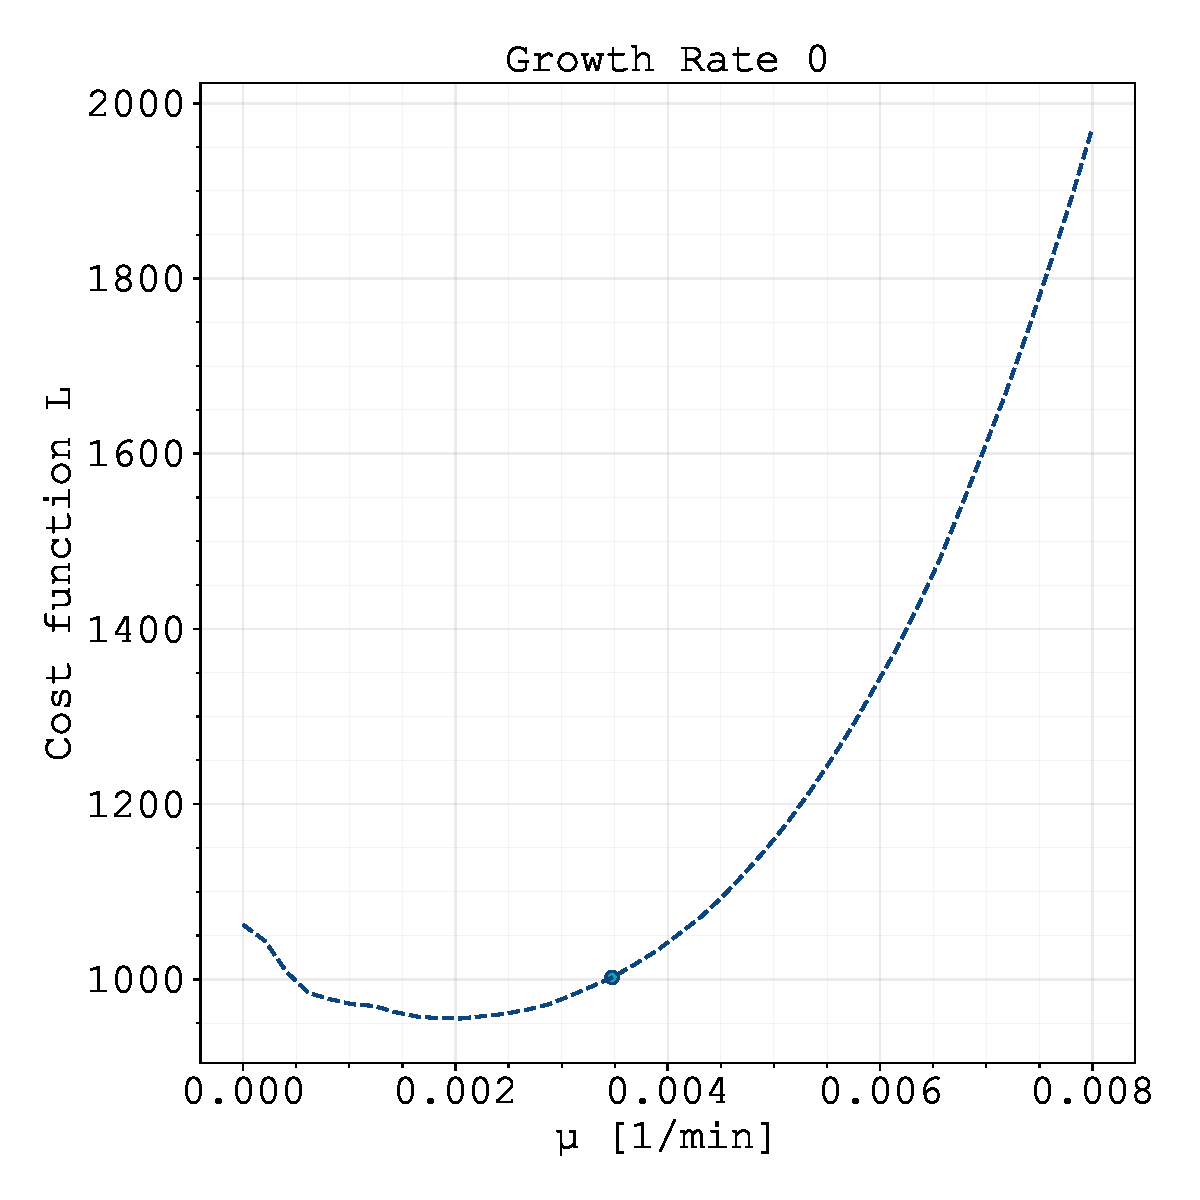
\includegraphics[width=0.33\textwidth]
        {figures/crm_fit/profiles/growth-rate-0.pdf}%
    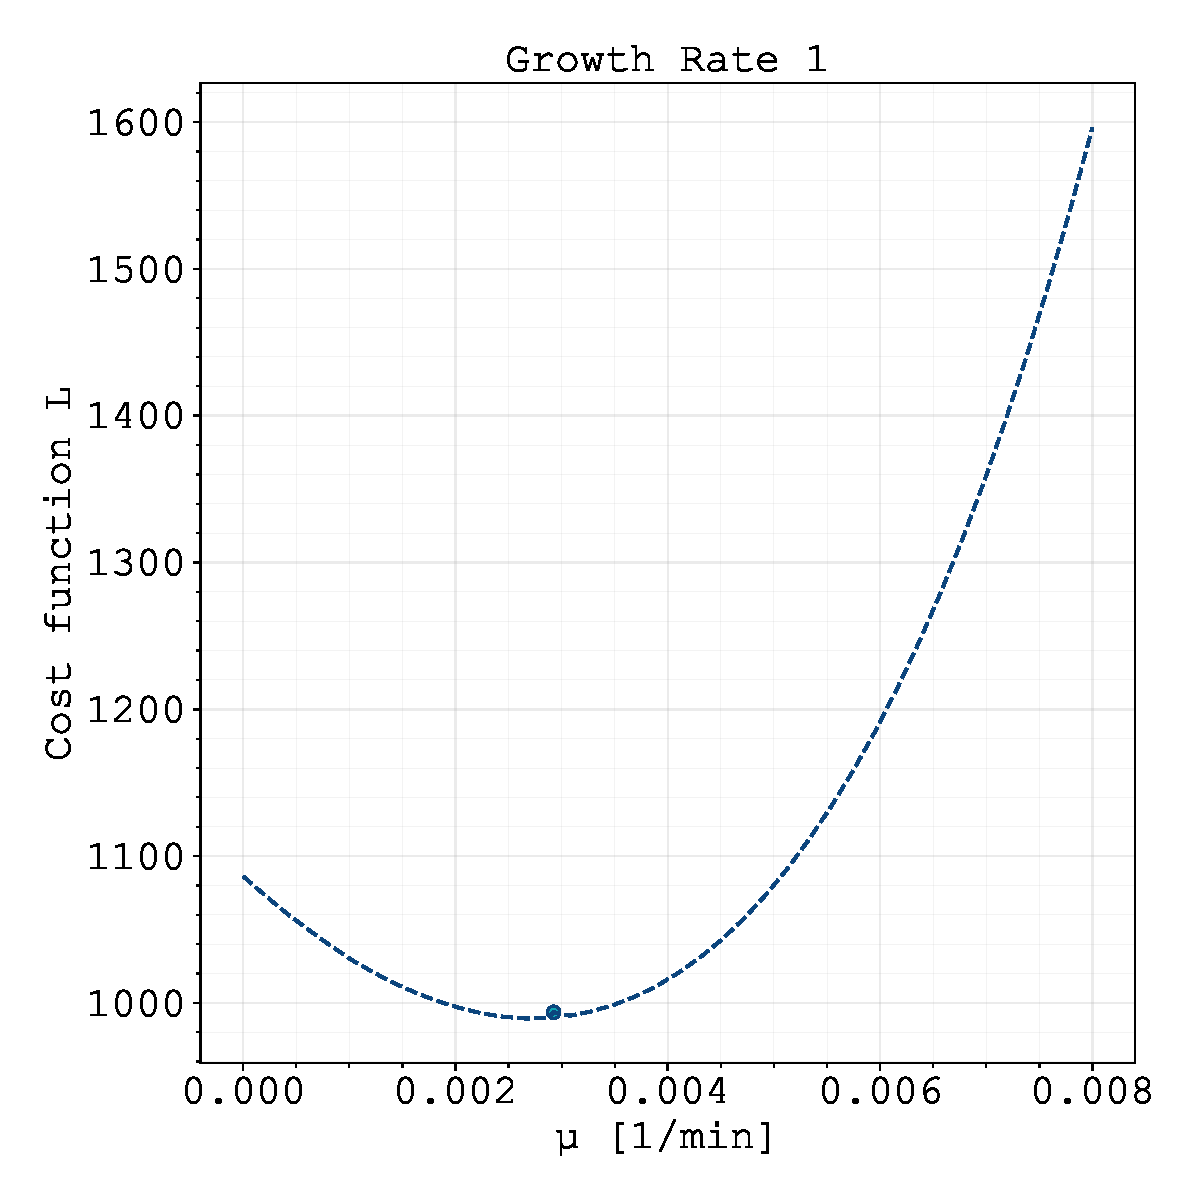
\includegraphics[width=0.33\textwidth]
        {figures/crm_fit/profiles/growth-rate-1.pdf}%
    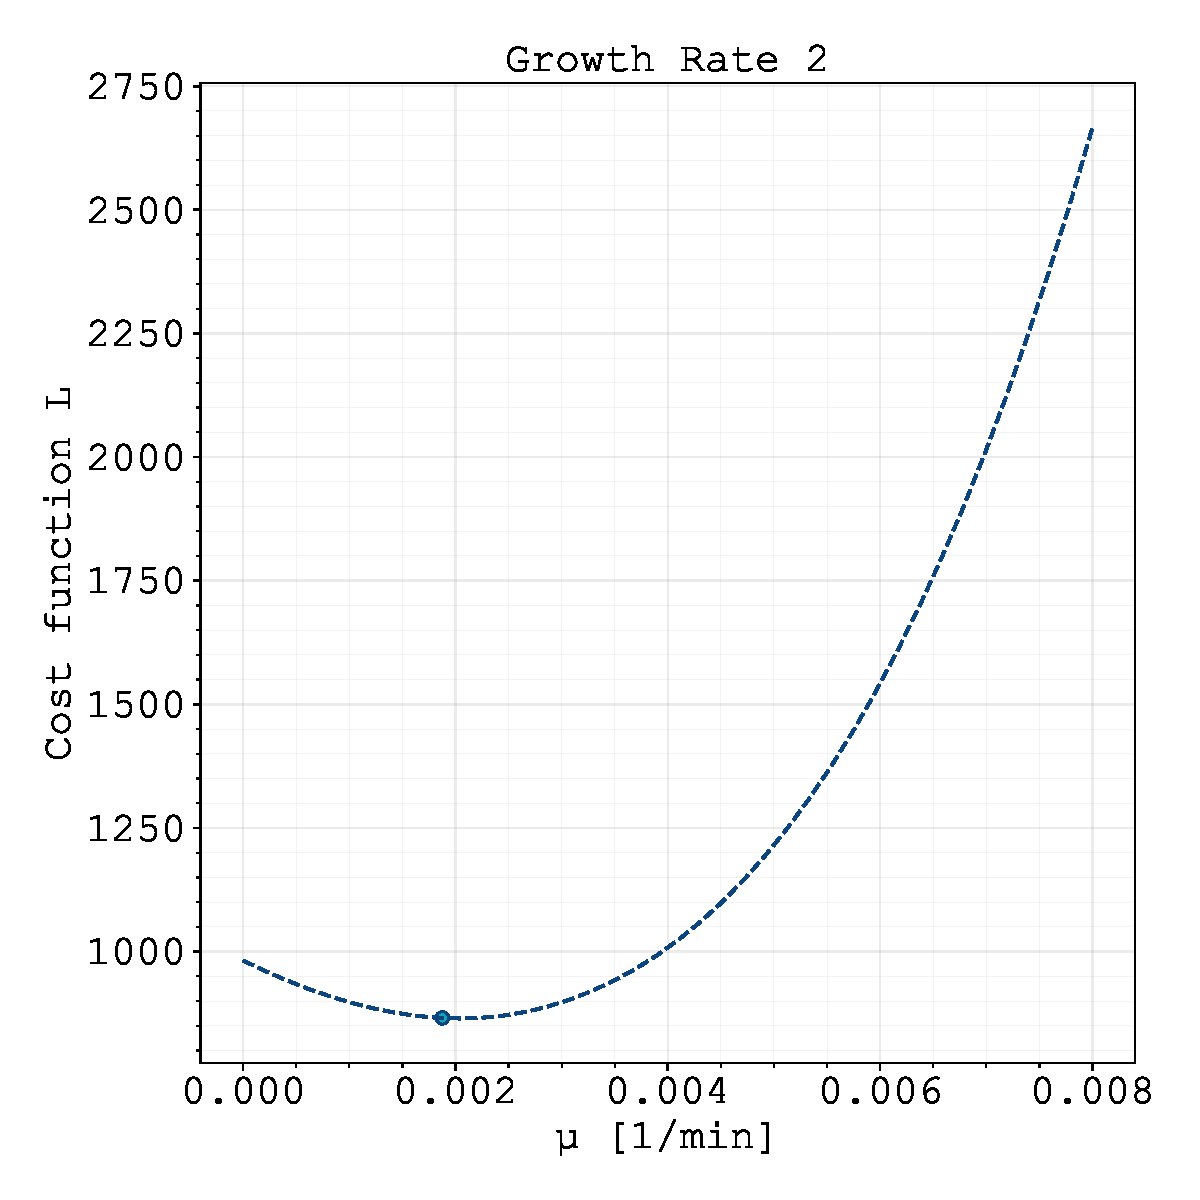
\includegraphics[width=0.33\textwidth]
        {figures/crm_fit/profiles/growth-rate-2.pdf}\\%
    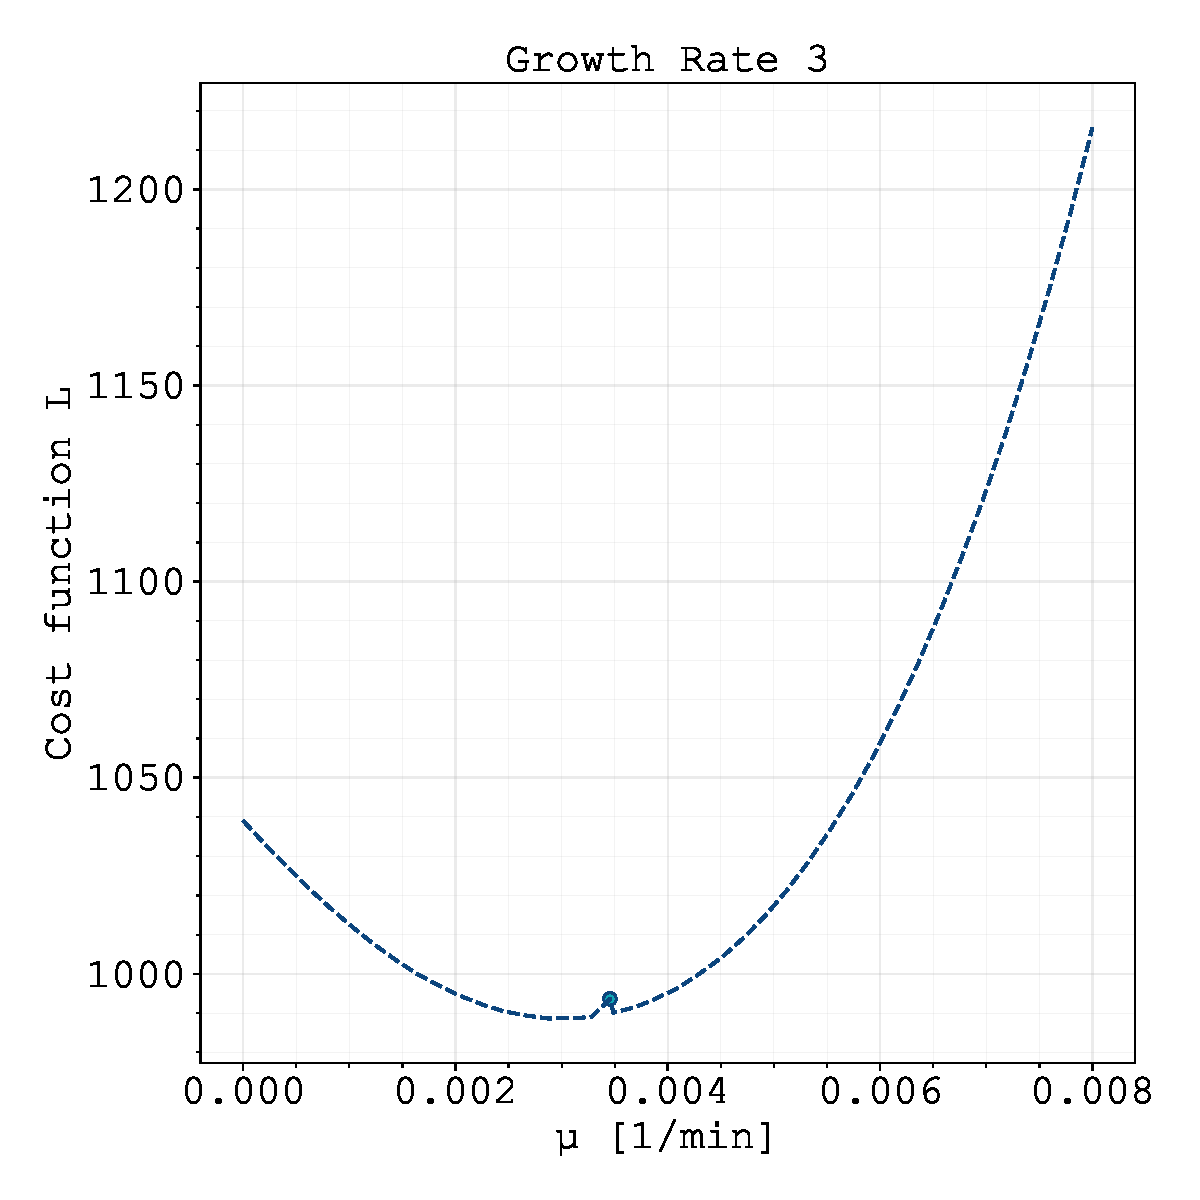
\includegraphics[width=0.33\textwidth]
        {figures/crm_fit/profiles/growth-rate-3.pdf}%
    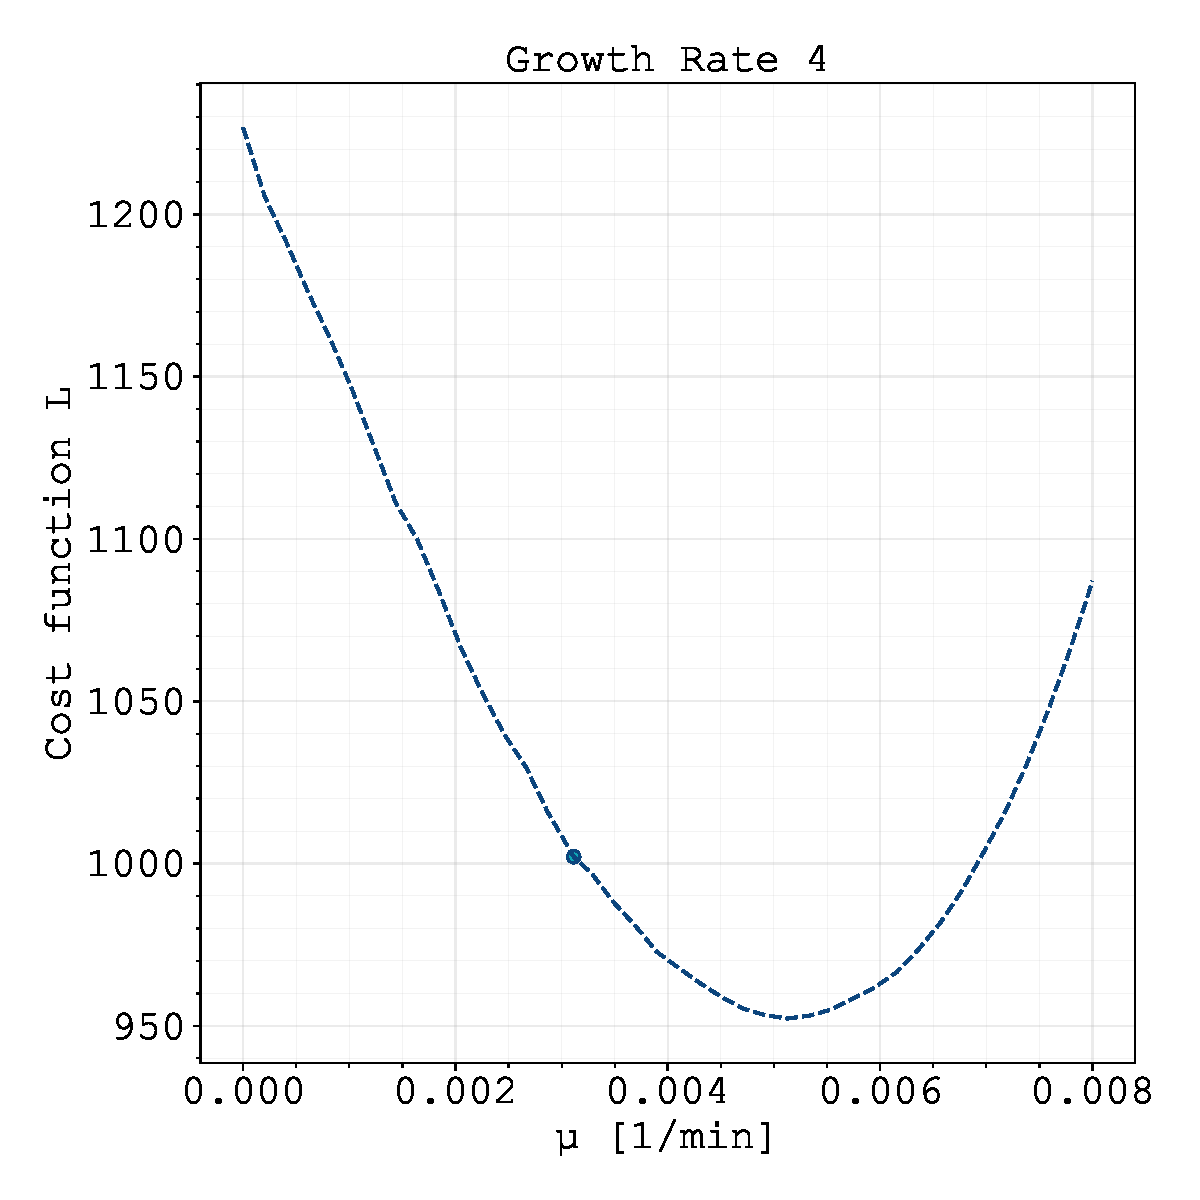
\includegraphics[width=0.33\textwidth]
        {figures/crm_fit/profiles/growth-rate-4.pdf}%
    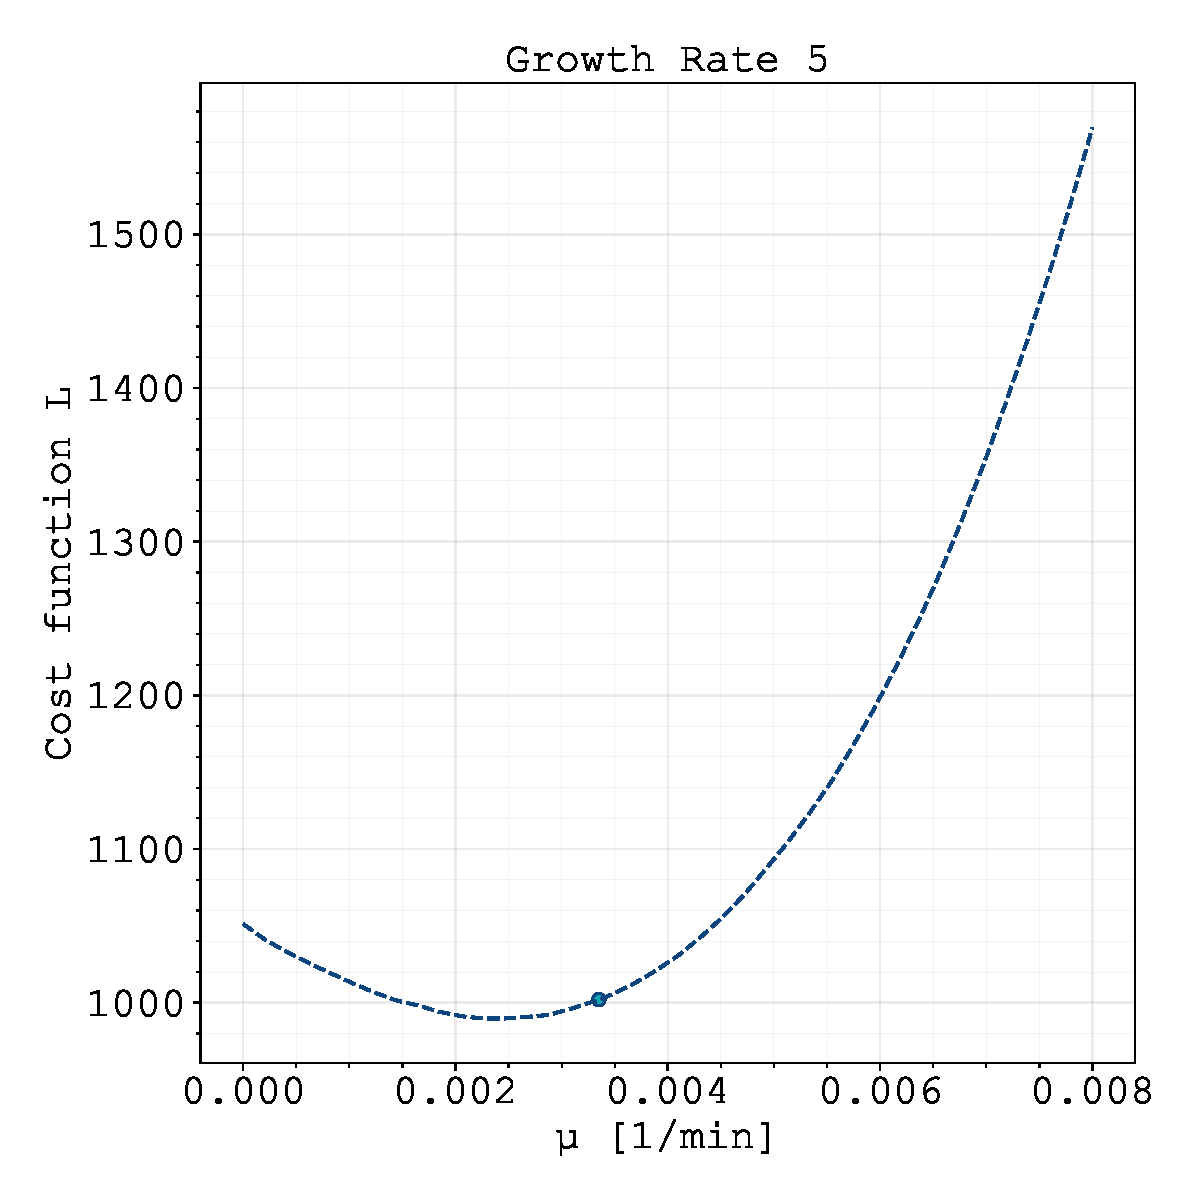
\includegraphics[width=0.33\textwidth]
        {figures/crm_fit/profiles/growth-rate-5.pdf}
    \caption{Parameter estimation of growth rates for individual cells}%TODO extend caption}
    \label{fig:parameter-estimates-supplement-growth-rates}
\end{figure}
\begin{figure}
    \centering
    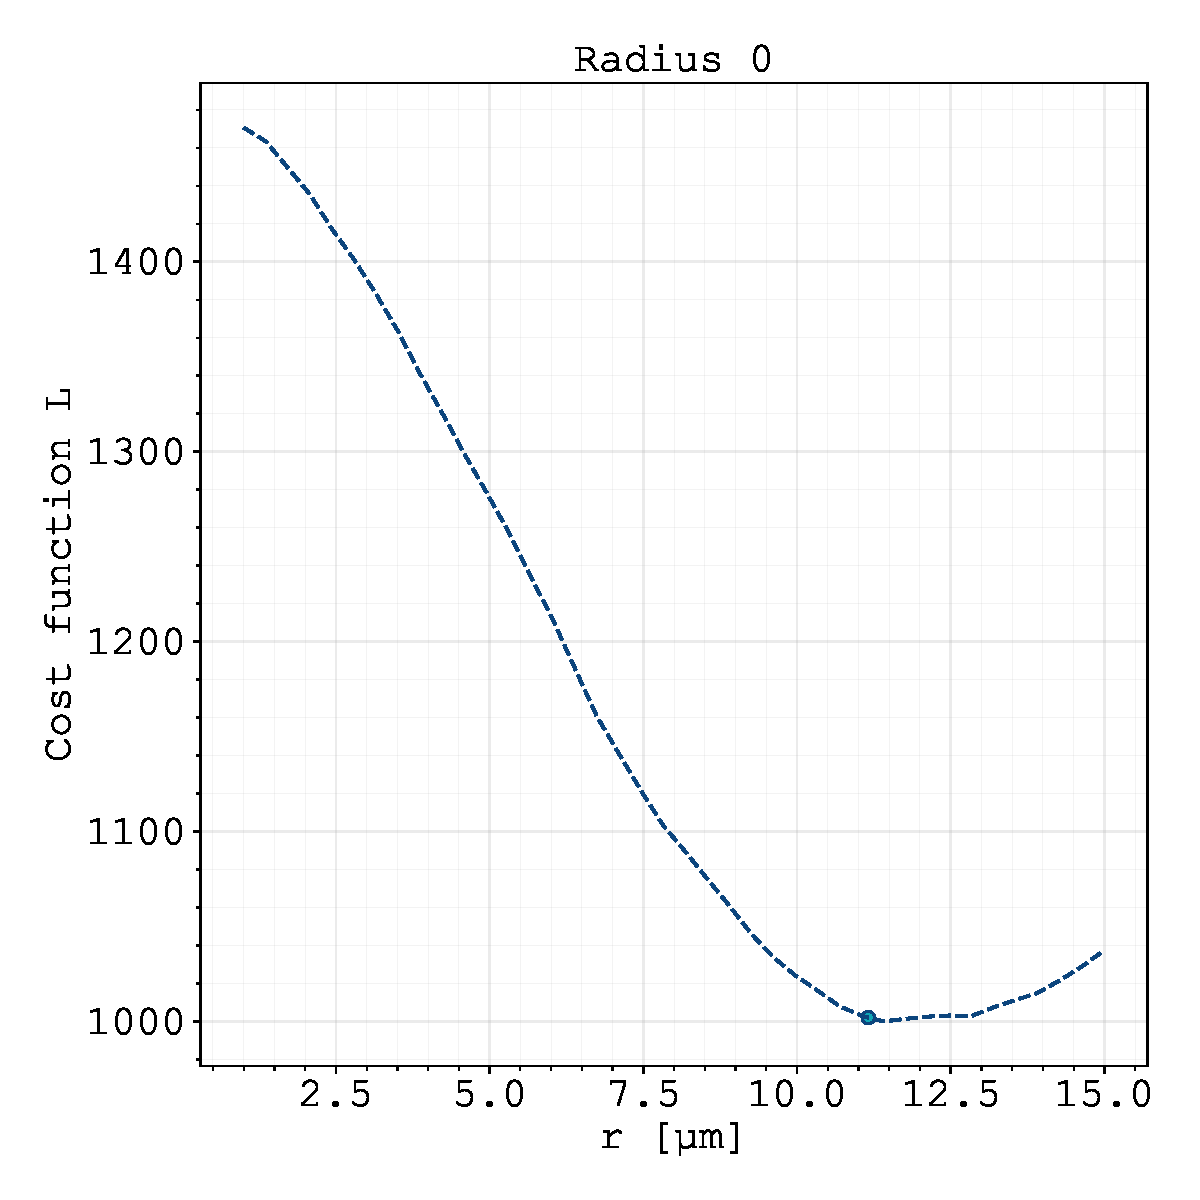
\includegraphics[width=0.33\textwidth]
        {figures/crm_fit/profiles/radius-0.pdf}%
    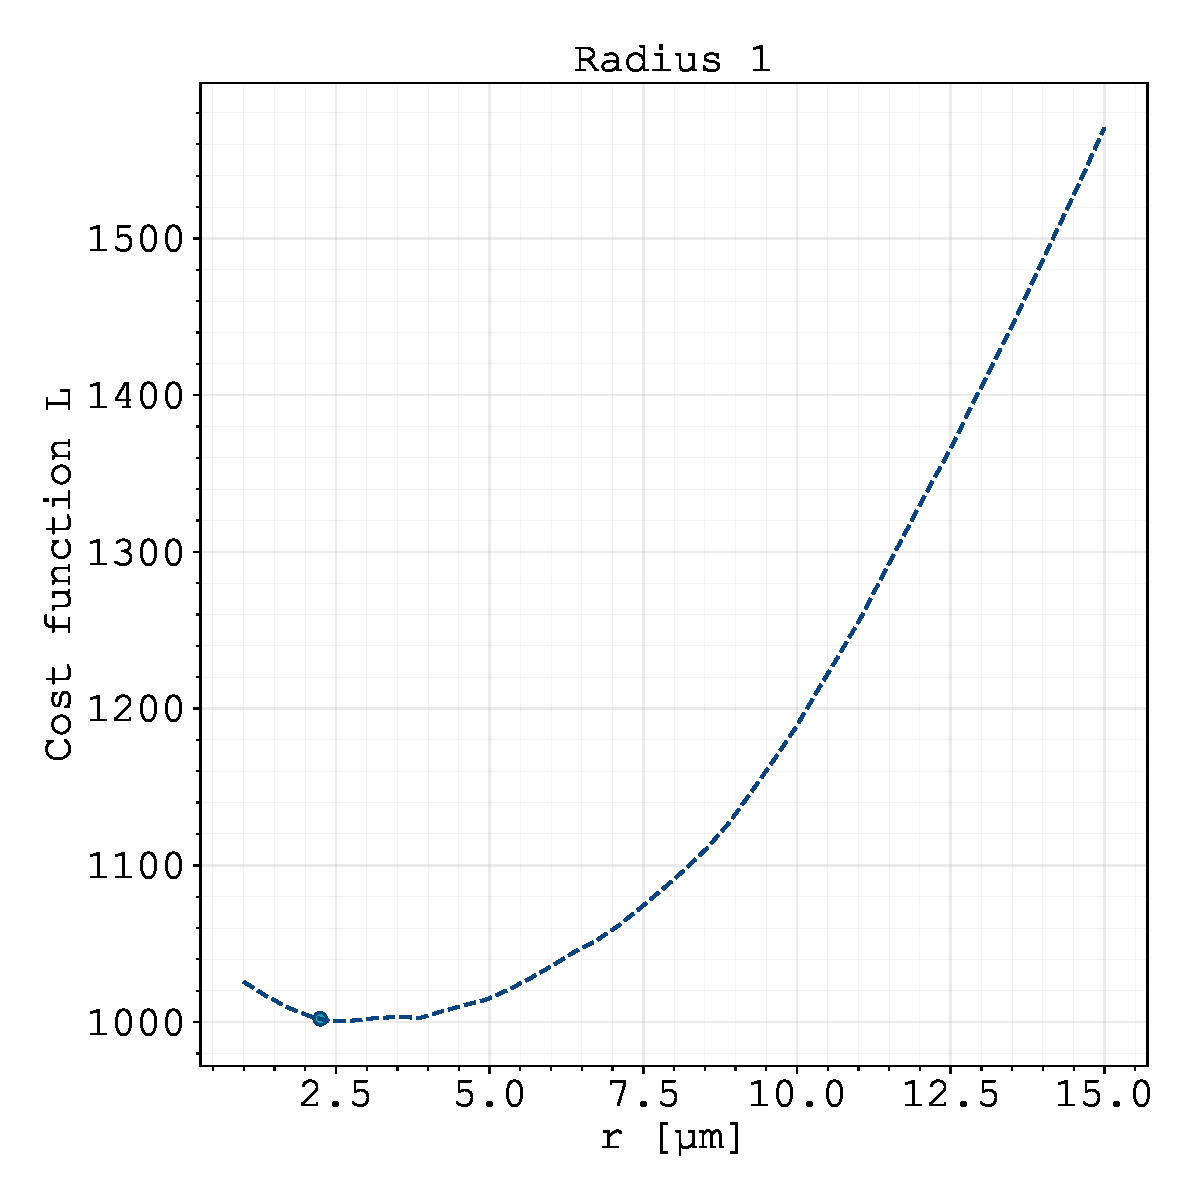
\includegraphics[width=0.33\textwidth]
        {figures/crm_fit/profiles/radius-1.pdf}%
    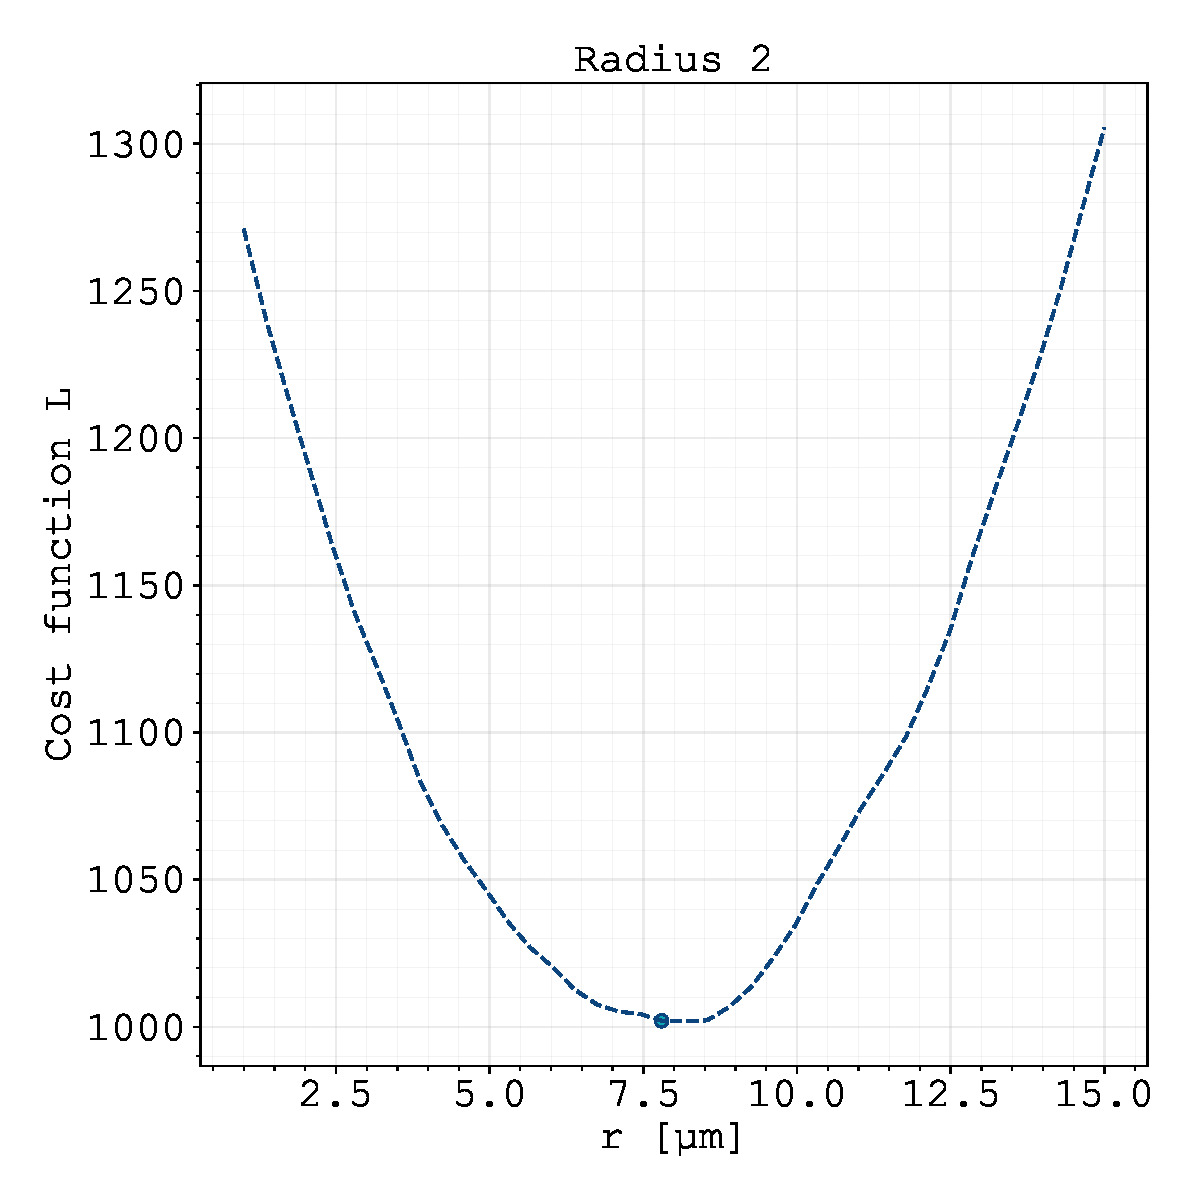
\includegraphics[width=0.33\textwidth]
        {figures/crm_fit/profiles/radius-2.pdf}\\%
    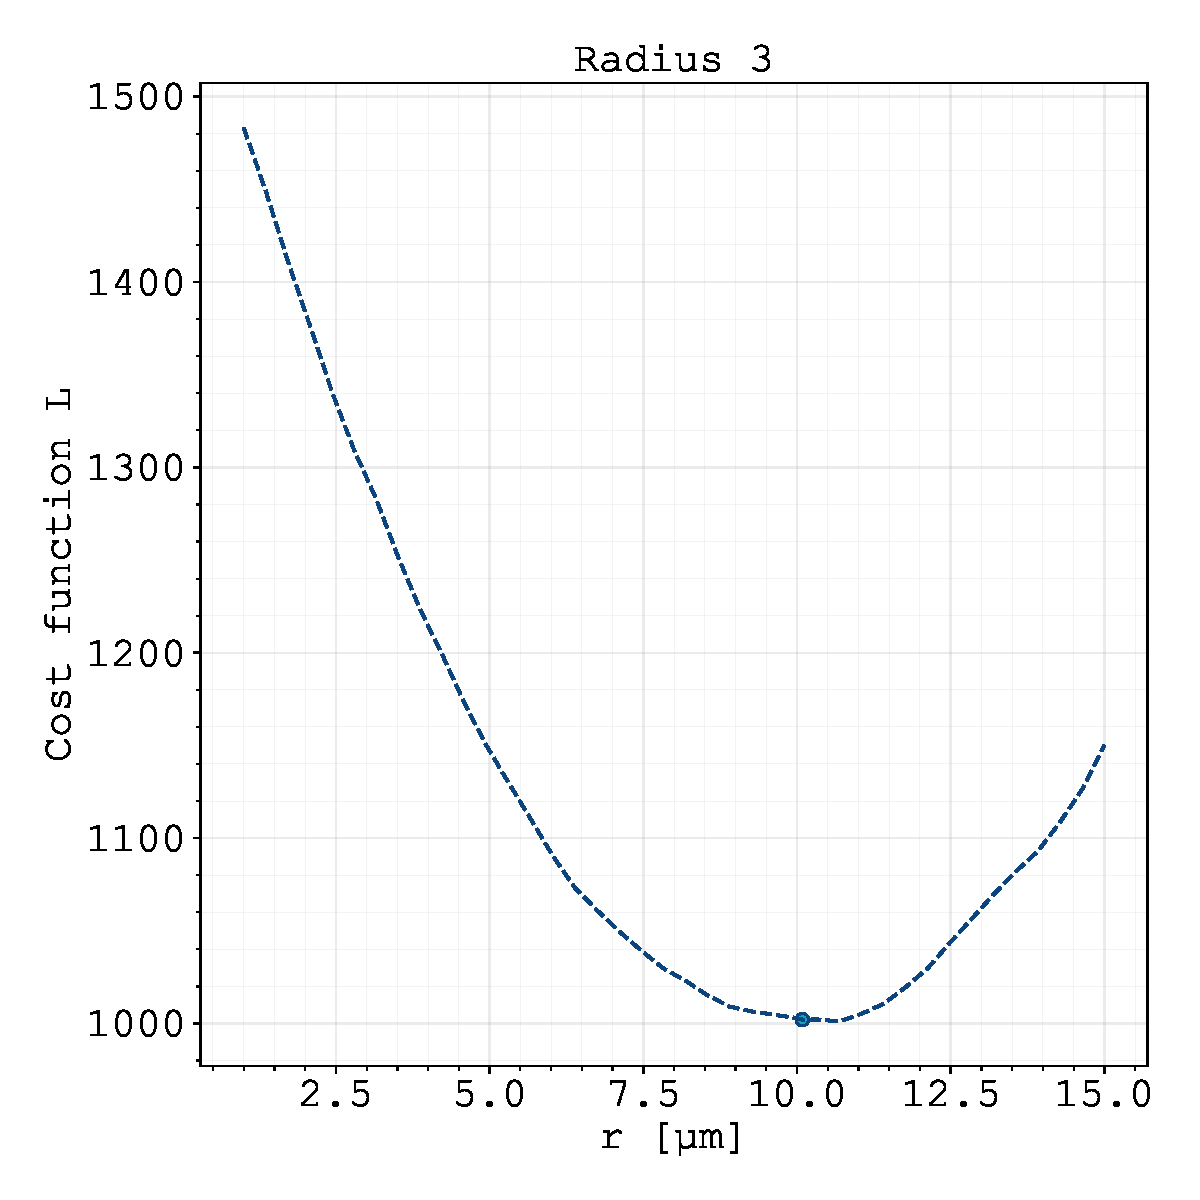
\includegraphics[width=0.33\textwidth]
        {figures/crm_fit/profiles/radius-3.pdf}%
    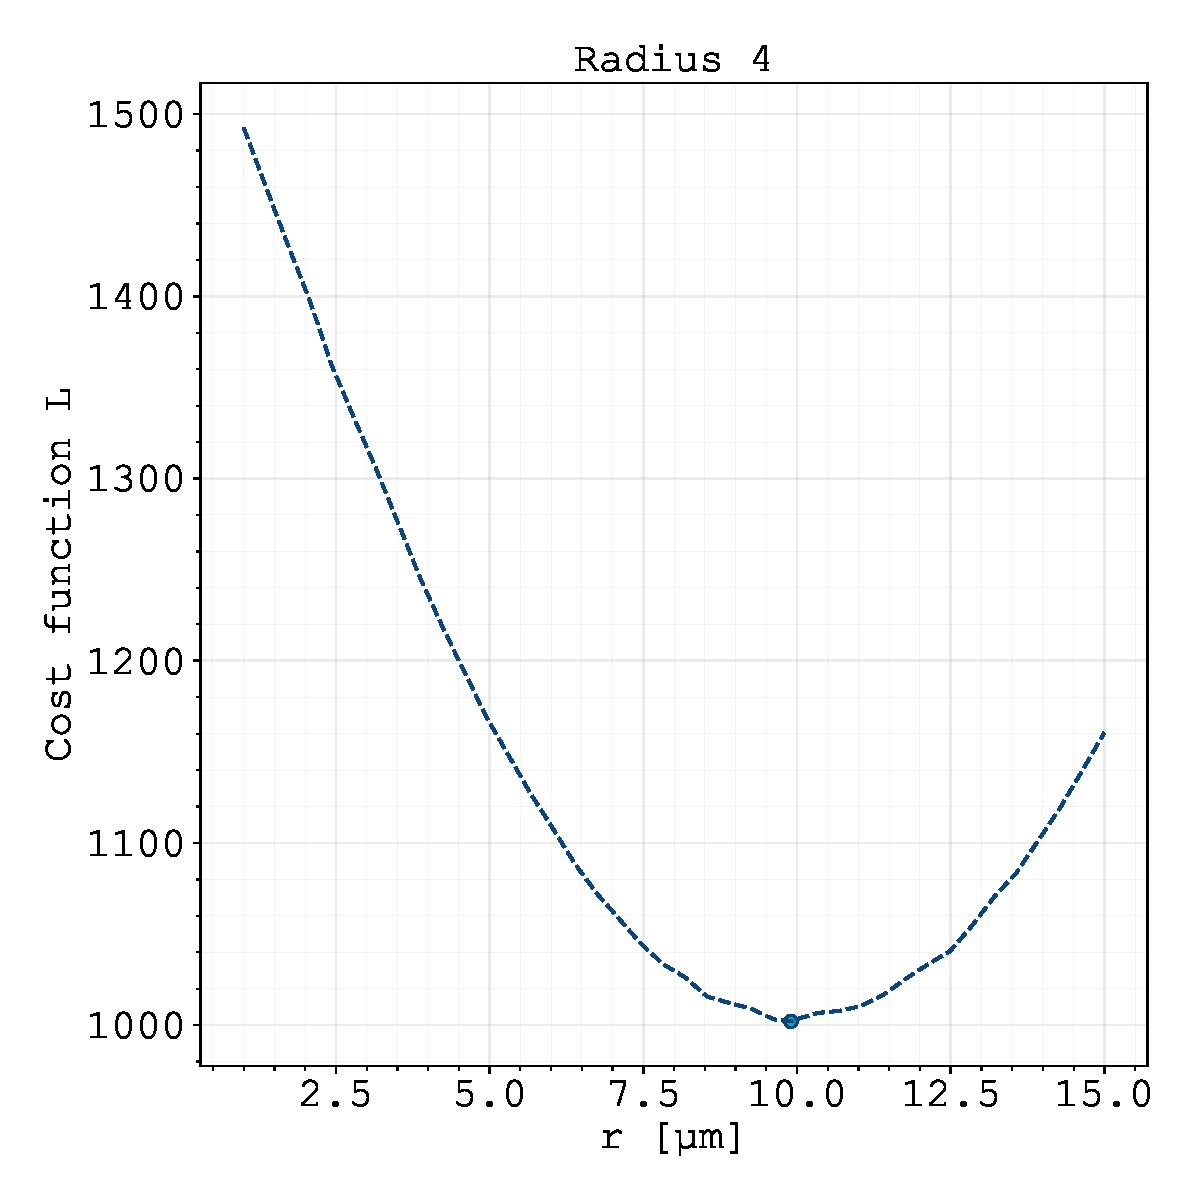
\includegraphics[width=0.33\textwidth]
        {figures/crm_fit/profiles/radius-4.pdf}%
    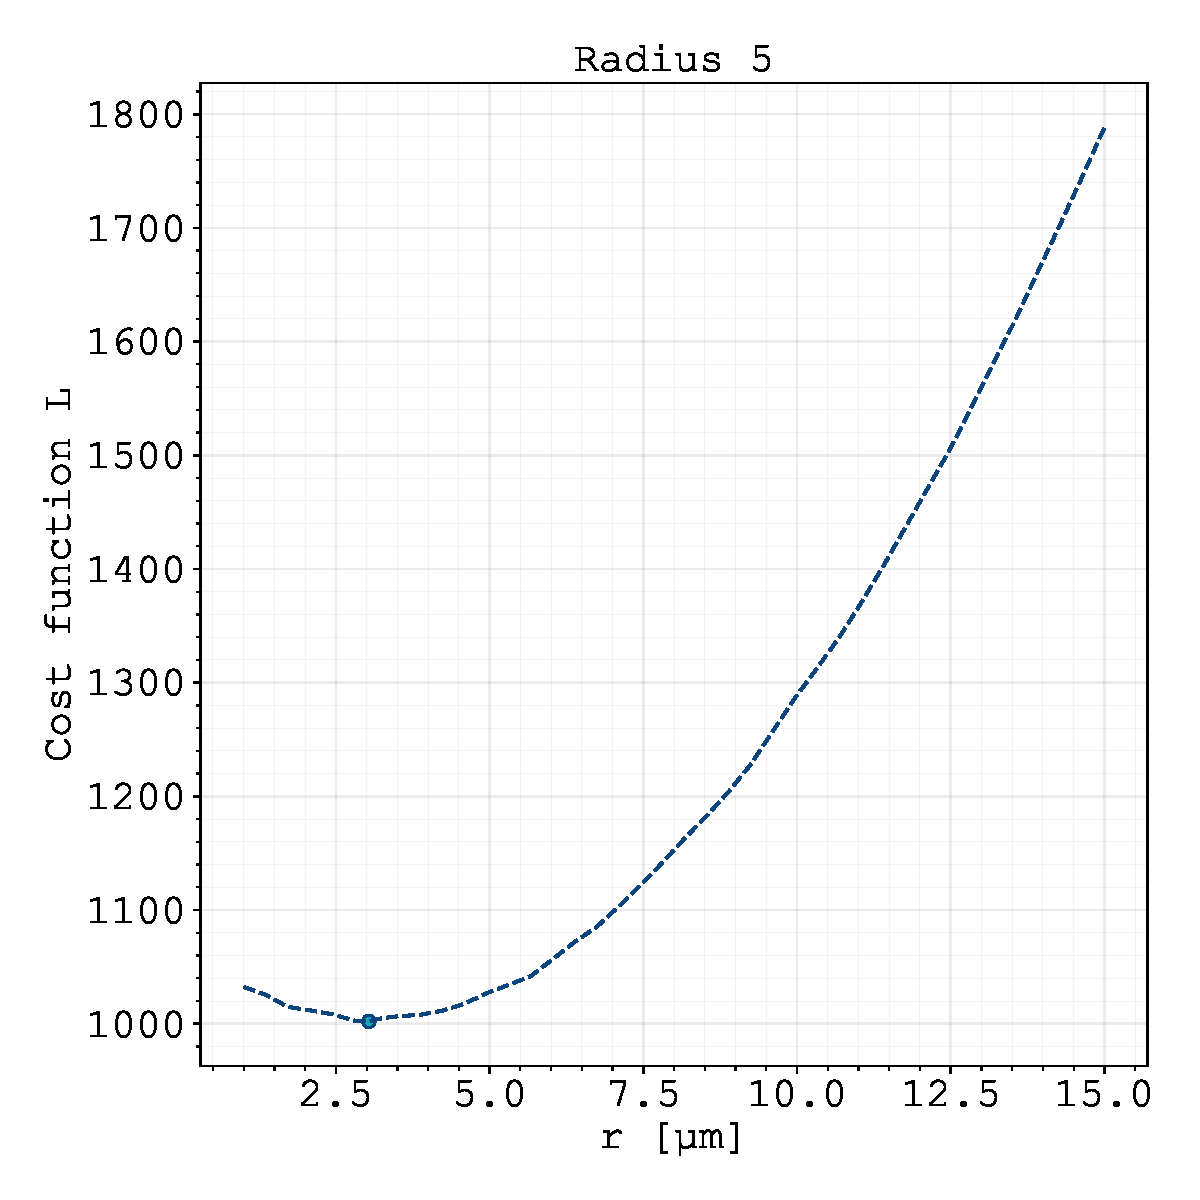
\includegraphics[width=0.33\textwidth]
        {figures/crm_fit/profiles/radius-5.pdf}%
    \caption{Parameter estimation of radii for individual cells}%TODO extend caption}
    \label{fig:parameter-estimates-supplement-radii}
\end{figure}

%###################################################################################################
\section{More Simulation Aspects}
\label{section:supplement-more-simulation-aspects}
%TODO insert this into the discussion later
\begin{table}[H]
    \centering
    \def\arraystretch{1.3}
    \begin{tabularx}{\textwidth}{c l X}
        &\textbf{Aspect} & \textbf{Description}\\
        \toprule
        &\textbf{(C) Cellular}\\
        \midrule
        (1) & Rod-Shaped Mechanics &
            Rod-shaped bacteria are flexible rods which are able to freely move around (off-lattice
            approach) \cite{Takeuchi2005,Ursell2014,Amir2014_2}.\\
        (2) & Growth &
            Cells grow exponentially by inserting new material either along the circular part of the
            rod or at the tip~\cite{Robert2014,Takeuchi2005}.\\
        (3) & Differentiation &
            \textit{B.subtilis} is known to differentiate into matrix-producing and
            surfactin-producing cells \cite{vanGestel2015,Lpez2010}.\\
        (4) & Division &
            The formation and continuation of van Gogh bundles is driven by cell division
            \cite{vanGestel2015}.
            Bacteria can form multilayers during their growth phase \cite{Duvernoy2018}.\\
        (5) & Variable Parameters &
            Parameters for individual cells are not fixed values but rather taken from a
            distribution \cite{Koutsoumanis2013}.\\
        &\textbf{(CC) Cell-Cell Interactions}\\
        \midrule
        (6) & Adhesion &
            Bacteria adhere to each other at longer distances and attach when in close contact
            \cite{Verwey1947,Trejo2013}.
            The interaction between rods can be polarized \cite{Duvernoy2018}.\\
        (7) & Friction &
            Friction between cells \cite{Grant2014} can be asymmetrical \cite{Doumic2020}.\\
        &\textbf{(DC) Domain-Cell Interactions}\\
        \midrule
        (8) & External Forces &
            Bacteria tend to stick to surfaces \cite{vanLoosdrecht1989}.
            The extracellular gel exerts a force onto the cells \cite{Grant2014}.\\
        (9) & Extracellular Reactions &
            Bacteria can take up nutrients or possible secrete/take up signalling molecules
            \cite{Li2025}.\\
        \bottomrule
    \end{tabularx}
    \label{table:simulation-aspects-supplement}
    \caption{
        This table extends table~\ref{table:simulation-aspects} with additional observations.
        It has to be noted that this table includes more specific behaviour that might not be
        generalizable across all types of rod-shaped bacteria.
    }
\end{table}

%###################################################################################################
\section{Performance}

\begin{itemize}
    \item Quadratic Scaling comes from more dense simulation
    \item Overall number of agents which can be simulated is satisfactory for current purposes
    \item Improvement from $1 \Rightarrow 2$ and $2\Rightarrow4$ threads; first is major; second
        only minor
    \item Flamegraph still shows much cycles running against hurdles::Barrier::wait $\Rightarrow$
        this leaves room for improvement
    \item Flamegraph also shows that $\approx 75\%$ of all cycles is related to actual work (not
        just waiting).
        In particular to update\_mechanics functions.
\end{itemize}

\begin{figure}
    \centering
    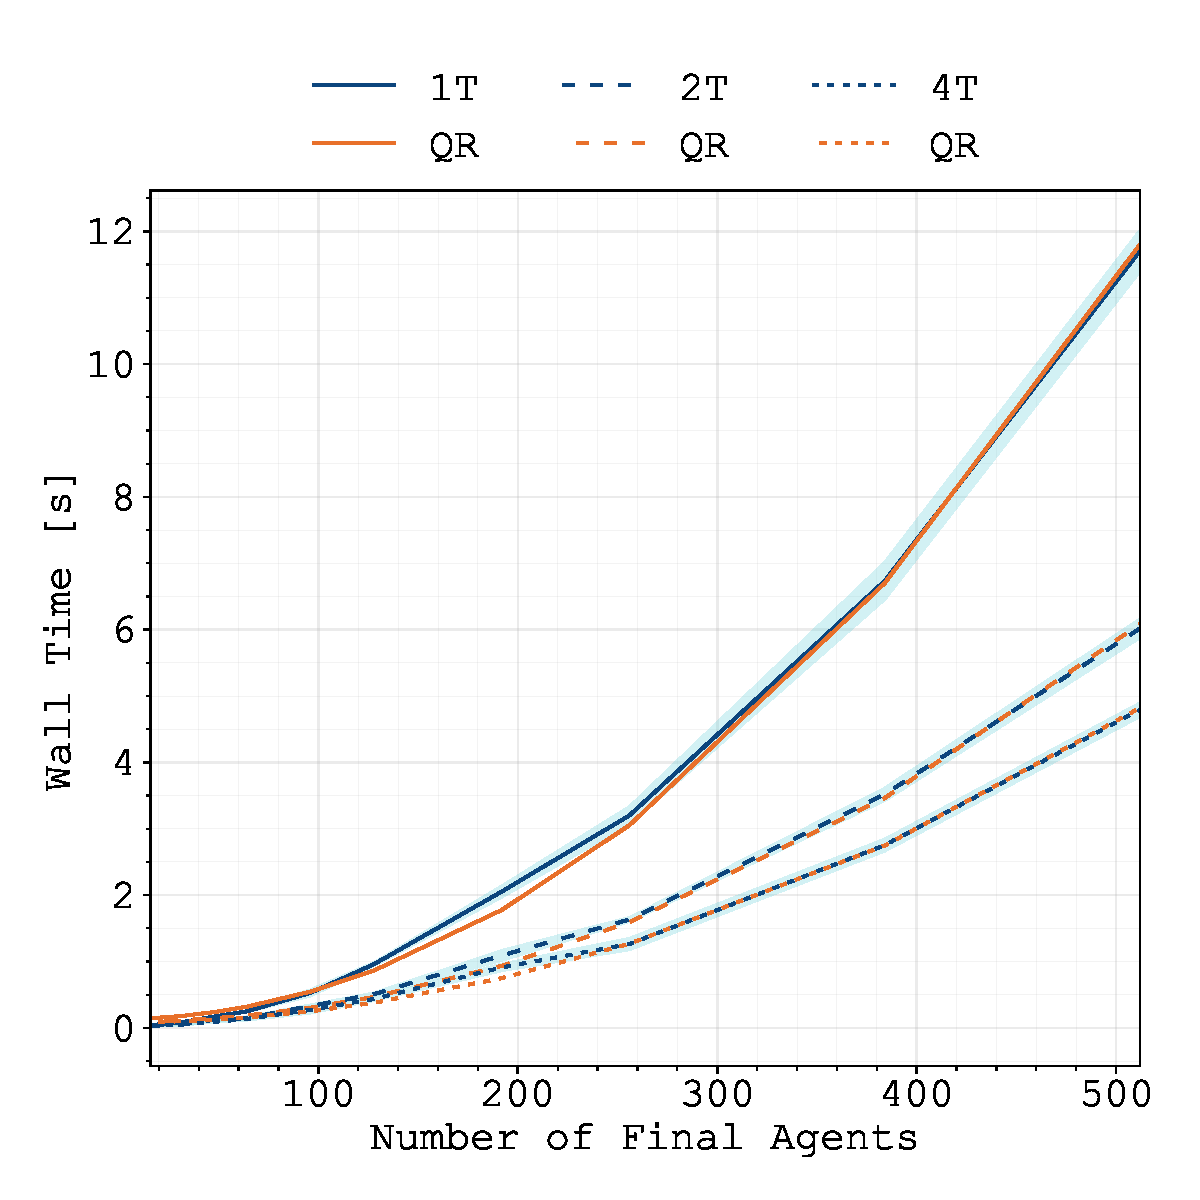
\includegraphics[width=0.49\textwidth]
        {docs/source/_static/performance/computation-time-with-initial-agents.pdf}
    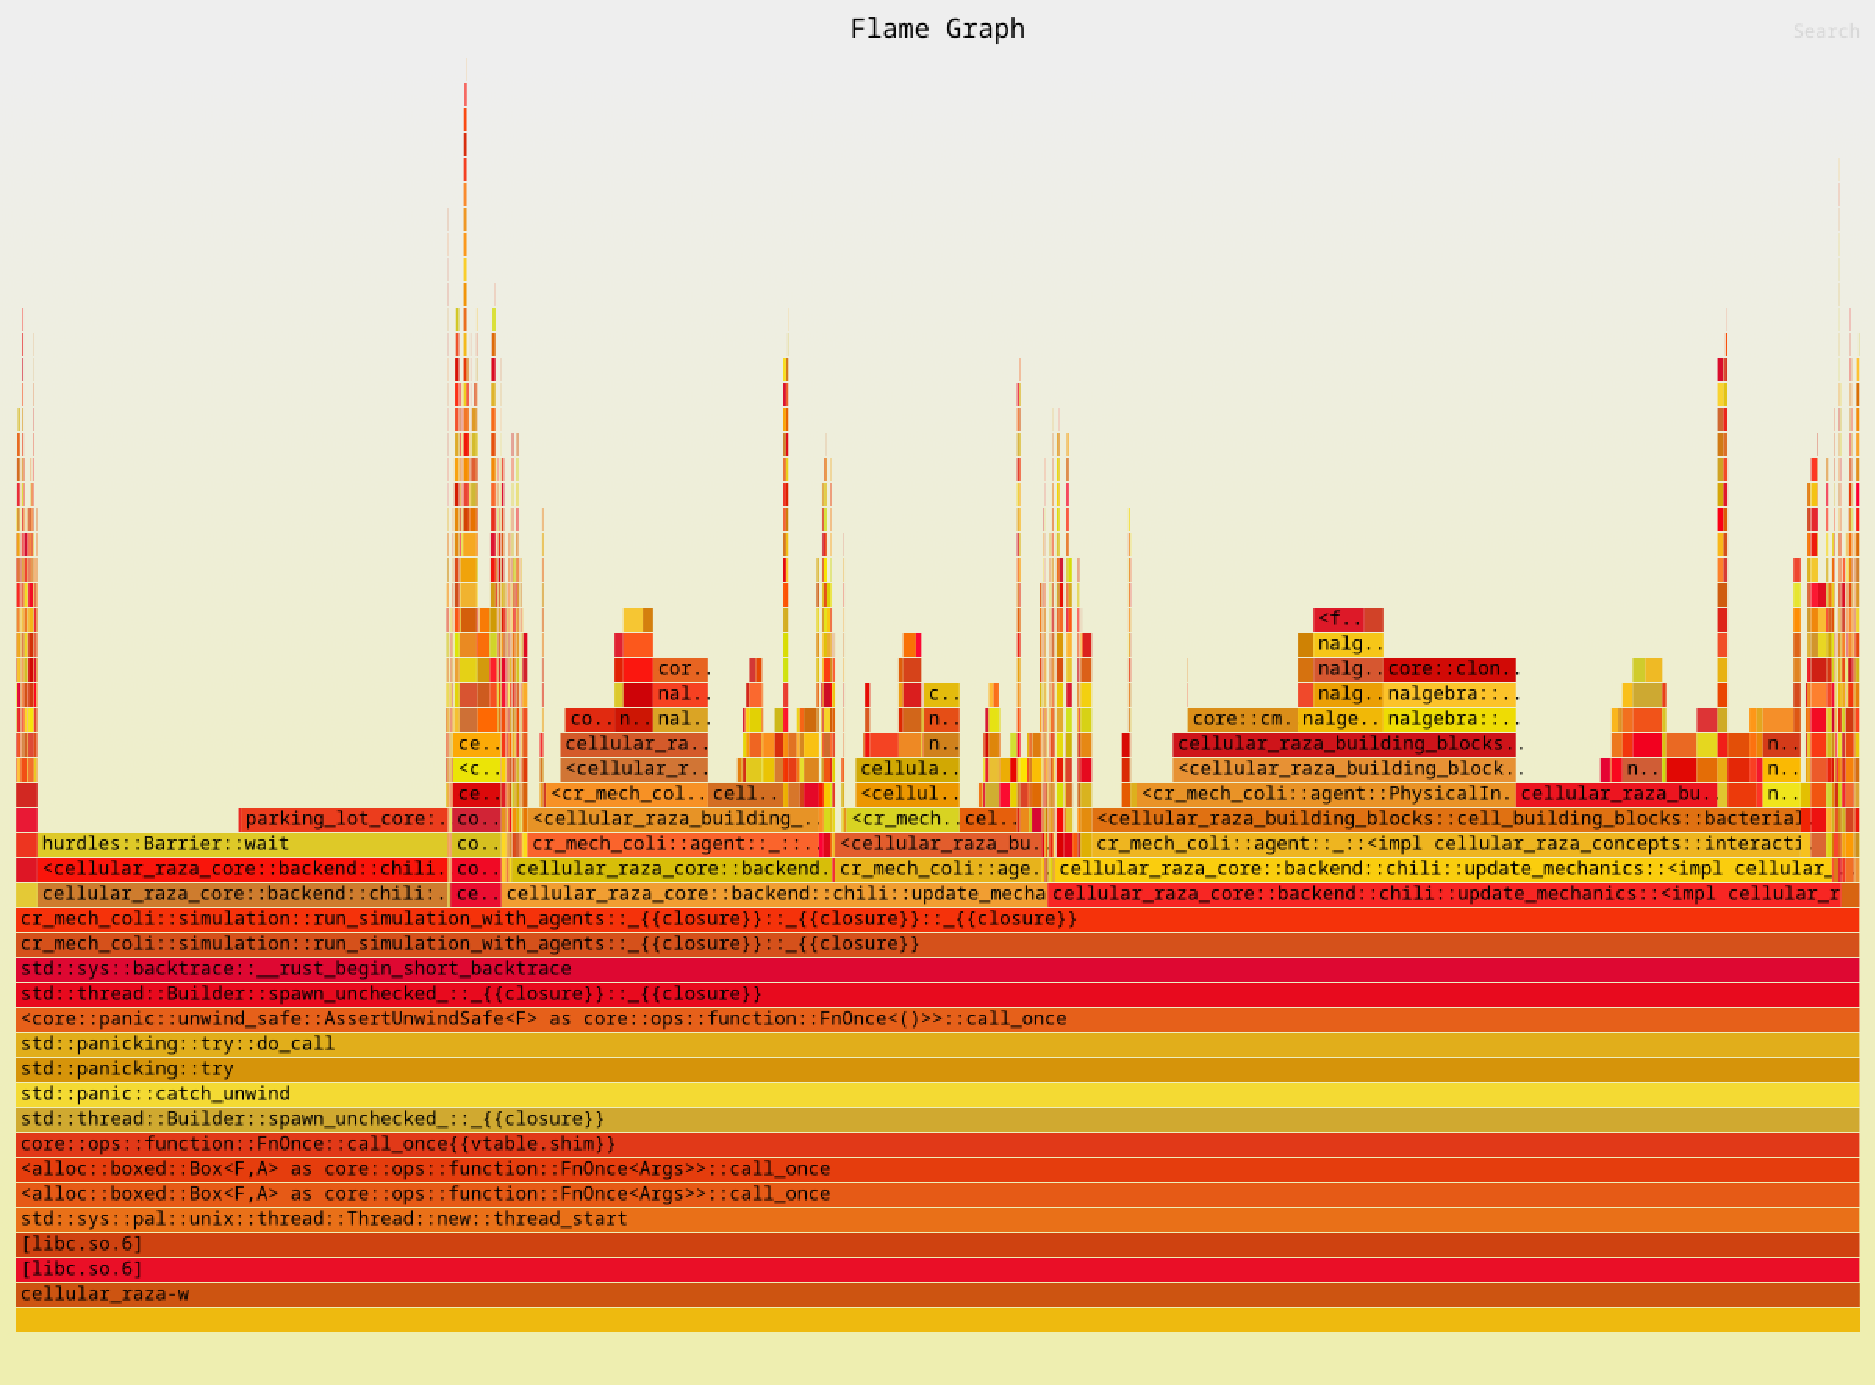
\includegraphics[width=0.49\textwidth]{docs/source/_static/performance/flamegraph.pdf}
    \caption{TODO}
    \label{fig:performance}
\end{figure}

%###################################################################################################
\section{Multilayer Predictions}
% TODO

\begin{itemize}
    \item Friction force against surface. perpendicular to motion; proportional to velocity.
    \item gel pressure coming from experiment (simply downwards force $F_z$)
\end{itemize}

\begin{itemize}
    \item Do we need this in this publication?
    \item Maybe this is out of scope as this is a more methodological paper.
    \item If we want to omit it, we might also opt to change the model description in the beginning
        and remove some parts of the external forces discussion.
\end{itemize}

\cite{You2019}

\begin{figure}
    \centering
    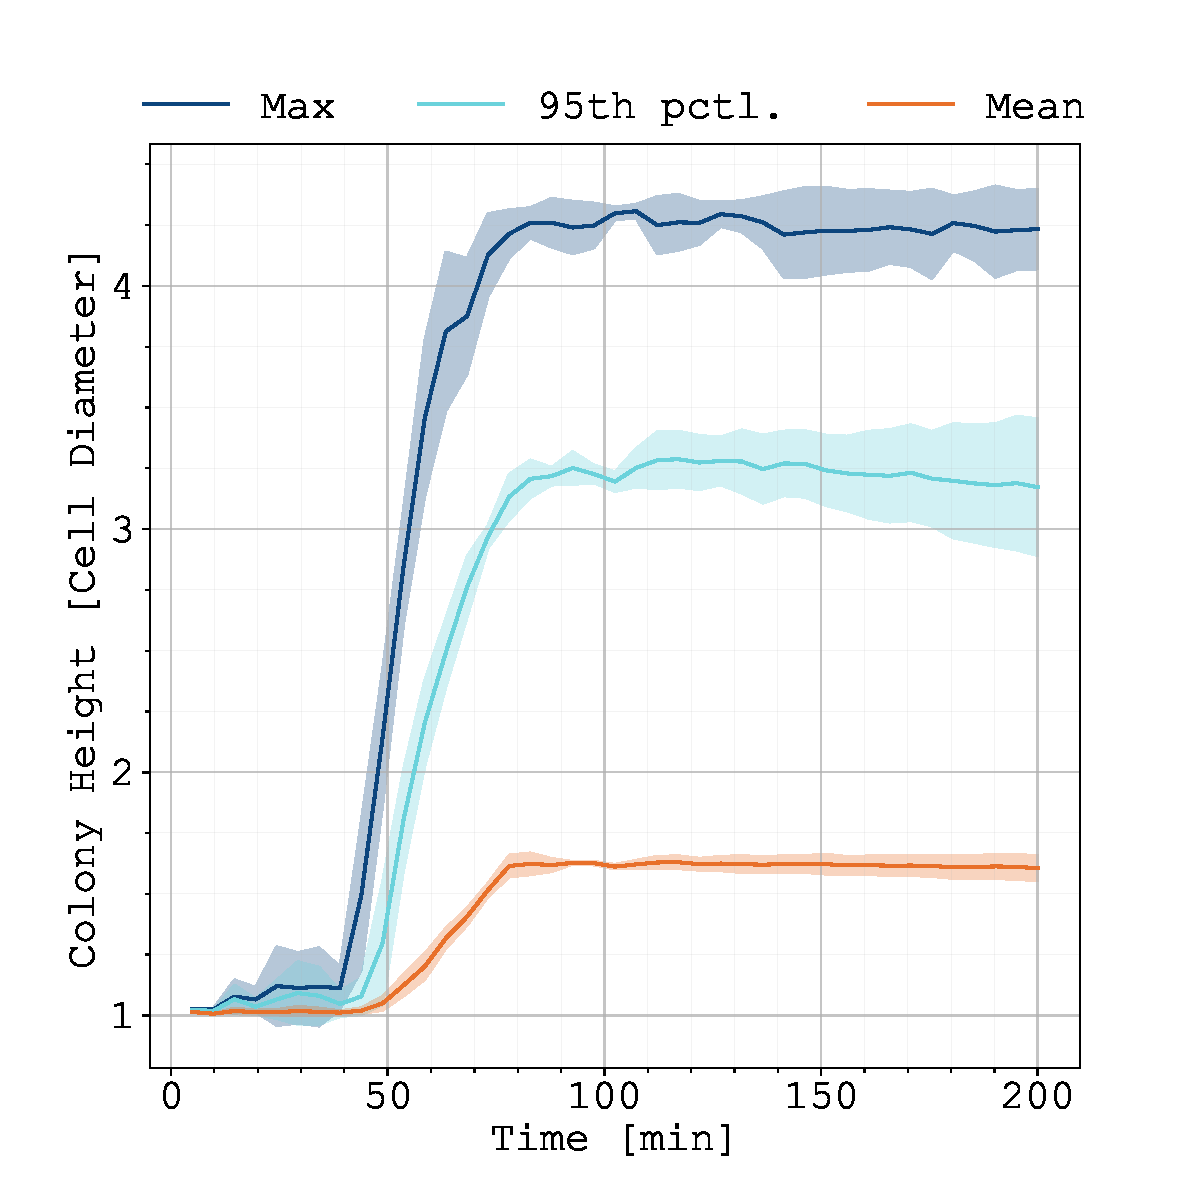
\includegraphics[width=0.49\textwidth]
        {docs/source/_static/scripts/crm_multilayer/multilayer-time-evolution.pdf}\\
    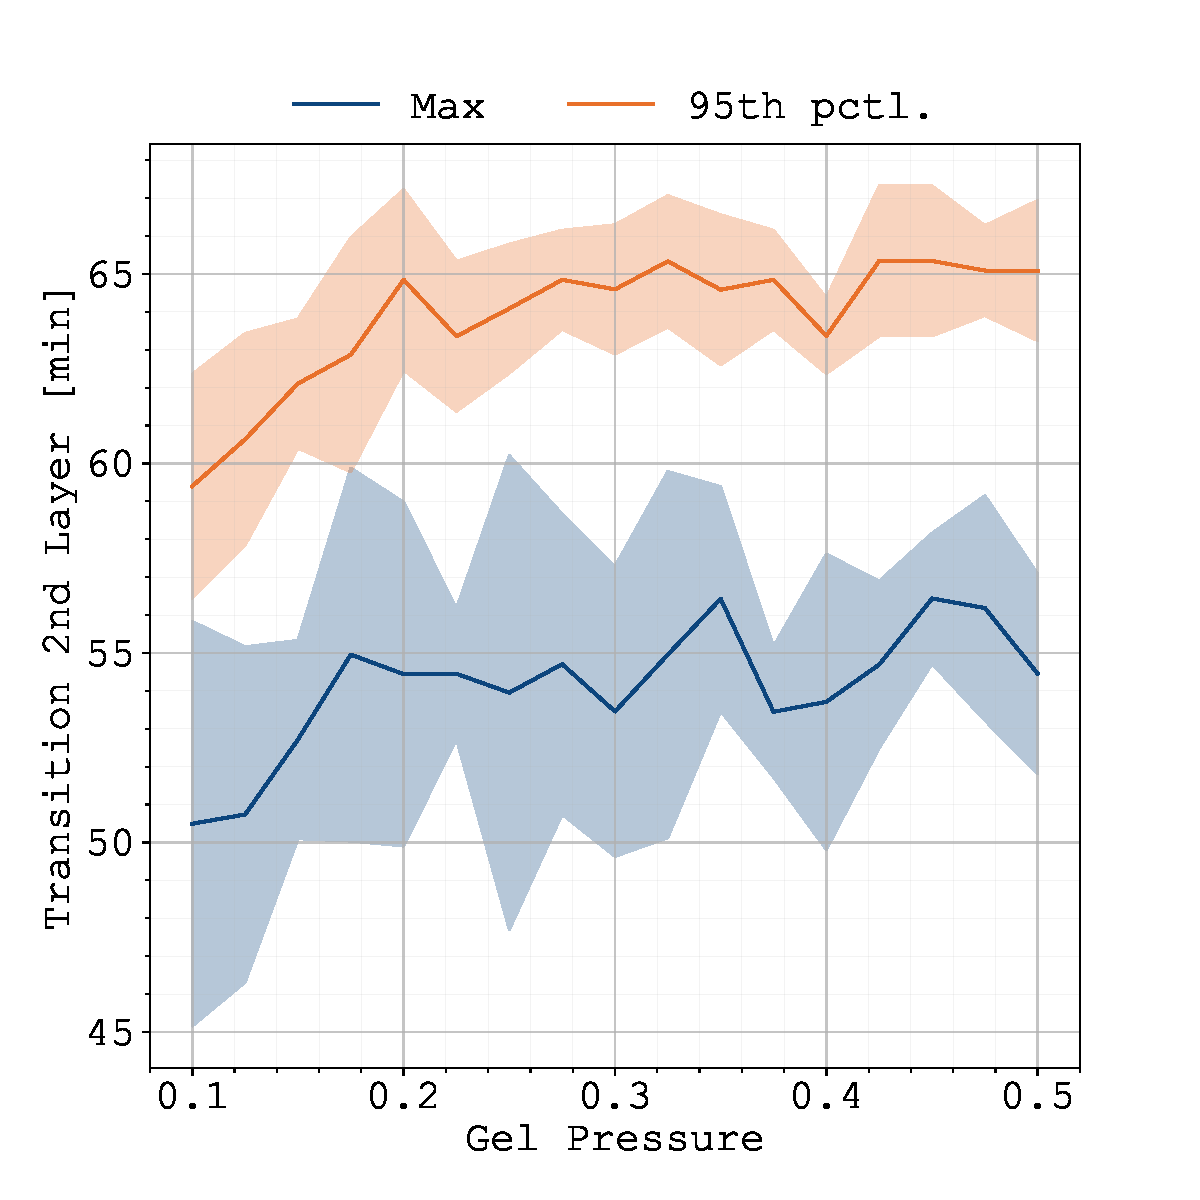
\includegraphics[width=0.49\textwidth]
        {docs/source/_static/scripts/crm_multilayer/colony-height-vs-gel_pressure.pdf}
    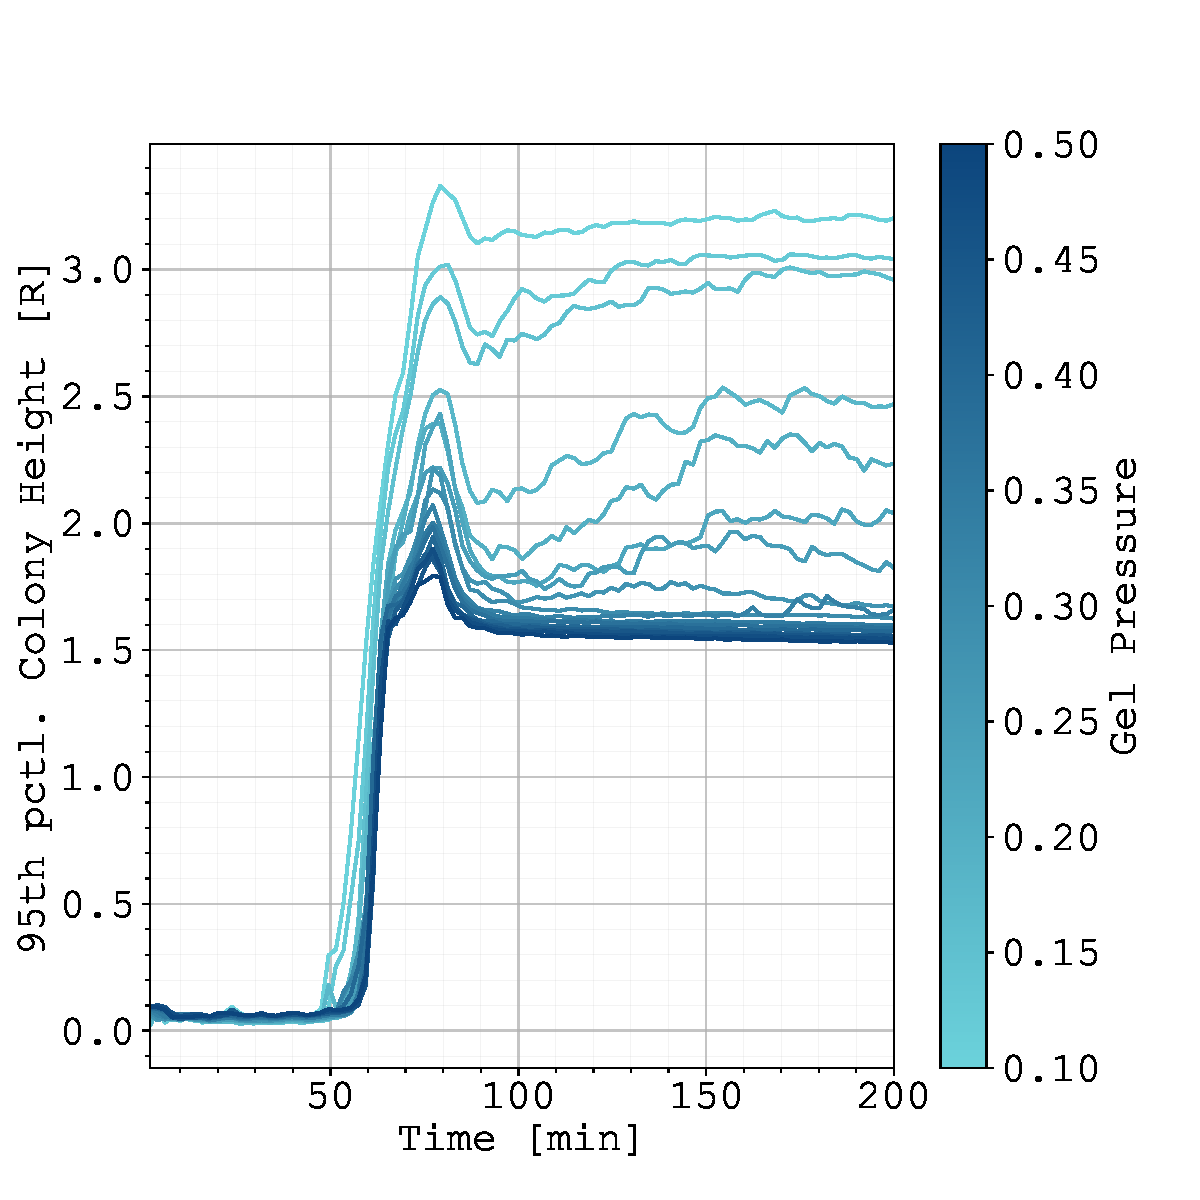
\includegraphics[width=0.49\textwidth]
        {docs/source/_static/scripts/crm_multilayer/colony-height-vs-time.pdf}
    \caption{TODO}
    \label{fig:multilayer}
\end{figure}


\end{document}
